\documentclass[11pt,a4paper]{article}
\usepackage[margin=2.2cm]{geometry}
\usepackage{booktabs,graphicx,parskip}
\usepackage[T1]{fontenc}
\usepackage{helvet}
\renewcommand{\familydefault}{\sfdefault}
\renewcommand{\thetable}{S\arabic{table}}
\renewcommand{\thefigure}{S\arabic{figure}}
\begin{document}
\begin{center}
{\large\bfseries Supplementary Information}\\[4pt]
Library size and sequence relatedness confound comparisons between synthetic
benchmarks and experimental antibody data\\[2pt]
Dohun Kim and Minho Bae
\end{center}
\vspace{1em}
\begin{table}[h]
\caption{Recovery of the top fraction of the library by guided and by random
search, before and after matching. The ratio is the quantity method papers
report; it falls from three digits to one once the library is matched in size
and structure.}
\centering
\begin{tabular}{@{}llrrr@{}}
\toprule
Library & Budget & Active & Random & Ratio \\
\midrule
Unmatched lattice, 6.9M & 500 & 0.121 & 0.000 & 627.25$\times$ \\
 & 2,000 & 0.547 & 0.000 & 1620.14$\times$ \\
 & 10,000 & 0.919 & 0.001 & 614.61$\times$ \\
Matched lattice, 6,000 & 200 & 0.030 & 0.030 & 1.00$\times$ \\
 & 500 & 0.440 & 0.070 & 6.29$\times$ \\
 & 1,000 & 0.663 & 0.200 & 3.32$\times$ \\
Measured, 6,000 & 200 & 0.033 & 0.033 & 1.00$\times$ \\
 & 500 & 0.256 & 0.087 & 2.95$\times$ \\
 & 1,000 & 0.434 & 0.145 & 2.99$\times$ \\
\bottomrule
\end{tabular}
\end{table}
\begin{table}[h]
\caption{One-hot encoding against ESM-2 embeddings on the matched library, over
twenty independent train/test splits. Negative values favour the language
model. Intervals are percentile bootstrap over splits; $p$-values are from a
one-sample $t$-test against zero, adjusted across the five sizes by the
Holm--Bonferroni and Benjamini--Hochberg procedures.}
\centering
\begin{tabular}{@{}rrrrrr@{}}
\toprule
Labels & Difference & 95\% CI & Raw $p$ & Holm $p$ & BH $p$ \\
\midrule
200 & -0.0365 & [-0.0447, -0.0284] & $5.6\times 10^{-8}$ & $2.8\times 10^{-7}$ & $2.8\times 10^{-7}$ \\
500 & -0.0181 & [-0.0231, -0.0126] & $2.3\times 10^{-6}$ & $9.4\times 10^{-6}$ & $5.9\times 10^{-6}$ \\
1,000 & -0.0071 & [-0.0098, -0.0043] & $7.7\times 10^{-5}$ & $2.3\times 10^{-4}$ & $1.3\times 10^{-4}$ \\
2,000 & -0.0009 & [-0.0018, 0.0001] & 0.084 & 0.168 & 0.105 \\
4,000 & 0.0000 & [-0.0006, 0.0007] & 0.919 & 0.919 & 0.919 \\
\bottomrule
\end{tabular}
\end{table}
\begin{table}[h]
\caption{Ridge regression against the max-pooling convolutional network on the
measured targets, over twelve splits for each of three targets. Positive values
favour ridge. The sign changes at 2,000 labels, the only size at which the two
are not separated after correction.}
\centering
\begin{tabular}{@{}rrrrr@{}}
\toprule
Labels & Difference & Raw $p$ & Holm $p$ & Separated \\
\midrule
200 & 0.0258 & $1.5\times 10^{-4}$ & $3.0\times 10^{-4}$ & yes \\
500 & 0.0308 & $1.5\times 10^{-10}$ & $6.2\times 10^{-10}$ & yes \\
1,000 & 0.0153 & $1.4\times 10^{-5}$ & $4.2\times 10^{-5}$ & yes \\
2,000 & -0.0015 & 0.507 & 0.507 & no \\
5,000 & -0.0182 & $4.9\times 10^{-13}$ & $2.5\times 10^{-12}$ & yes \\
10,000 & -0.0255 & $1.3\times 10^{-14}$ & $7.8\times 10^{-14}$ & yes \\
20,000 & -0.0266 & $3.7\times 10^{-15}$ & $2.6\times 10^{-14}$ & yes \\
\bottomrule
\end{tabular}
\end{table}
\begin{table}[h]
\caption{The third-party prospective campaign. Candidates from generators that
differ only in featurisation were all measured by AlphaSeq. Negative values
mean the language model produced the better candidates.}
\centering
\begin{tabular}{@{}llrrr@{}}
\toprule
Target & Comparison & Median difference & Raw $p$ & Holm $p$ \\
\midrule
aab-pp489 & esm warm vs ohe warm & -0.239 & $4.2\times 10^{-277}$ & $8.3\times 10^{-277}$ \\
aab-pp489 & esm cold vs ohe cold & -0.311 & $<10^{-300}$ & $<10^{-300}$ \\
pembrolizumab-scfv & esm warm vs ohe warm & -0.571 & $<10^{-300}$ & $<10^{-300}$ \\
pembrolizumab-scfv & esm cold vs ohe cold & -2.177 & $<10^{-300}$ & $<10^{-300}$ \\
vhh72 & esm warm vs ohe warm & -0.528 & $2.6\times 10^{-249}$ & $2.6\times 10^{-249}$ \\
vhh72 & esm cold vs ohe cold & -0.404 & $<10^{-300}$ & $<10^{-300}$ \\
\bottomrule
\end{tabular}
\end{table}
\begin{table}[h]
\caption{Seven models on the four measured targets, at the largest training-set
size for which every target is present. Intervals are a percentile bootstrap
that resamples targets rather than predictions, since nested subsets of one
dataset are not independent observations.}
\centering
\begin{tabular}{@{}lrr@{}}
\toprule
Model & Spearman & 95\% CI \\
\midrule
Ridge, ESM-2 + one-hot & 0.648 & [0.584, 0.716] \\
Ridge, ESM-2 & 0.639 & [0.578, 0.702] \\
Ridge, one-hot & 0.626 & [0.548, 0.709] \\
Convolutional network & 0.576 & [0.471, 0.680] \\
Random forest & 0.533 & [0.461, 0.599] \\
Boosted trees & 0.526 & [0.476, 0.575] \\
$k$-nearest neighbours (Hamming), control & 0.328 & [0.265, 0.391] \\
\bottomrule
\end{tabular}
\end{table}
\clearpage
\begin{figure}[h]
\centering
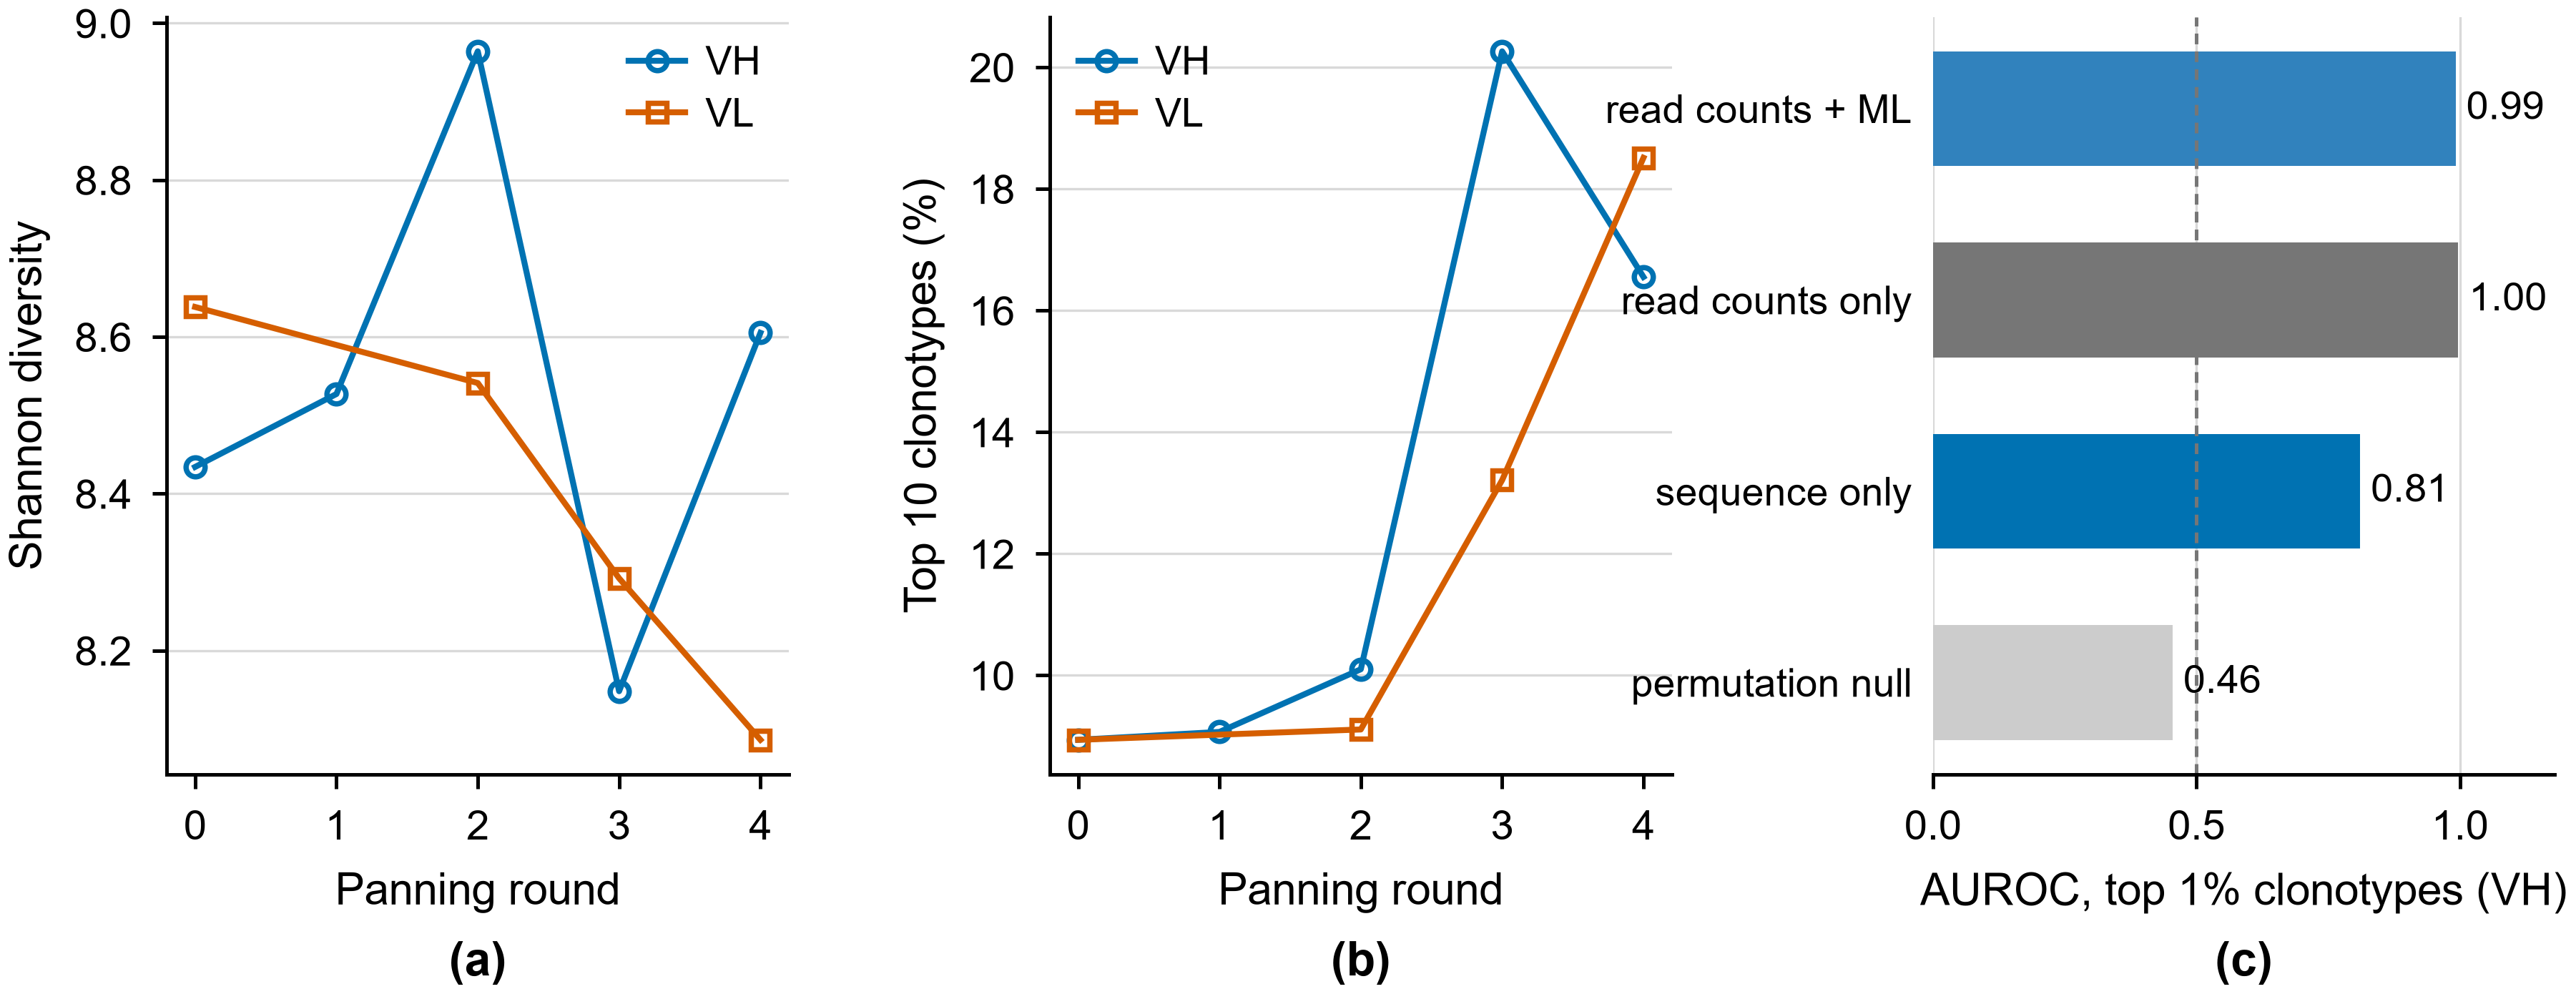
\includegraphics[width=\textwidth]{figs/SFig1.png}
\caption{Re-analysis of a five-round panning campaign. \textbf{(a)},
\textbf{(b)}, diversity and concentration by round, computed after rarefying to
equal depth and excluding clonotypes seen fewer than five times.
\textbf{(c)}, ability to identify the top 1\% of final-round clonotypes. Models
using read counts do not improve on ranking by the last available round, whereas
sequence alone carries signal well above the permutation null.}
\end{figure}

\begin{figure}[t]
\centering
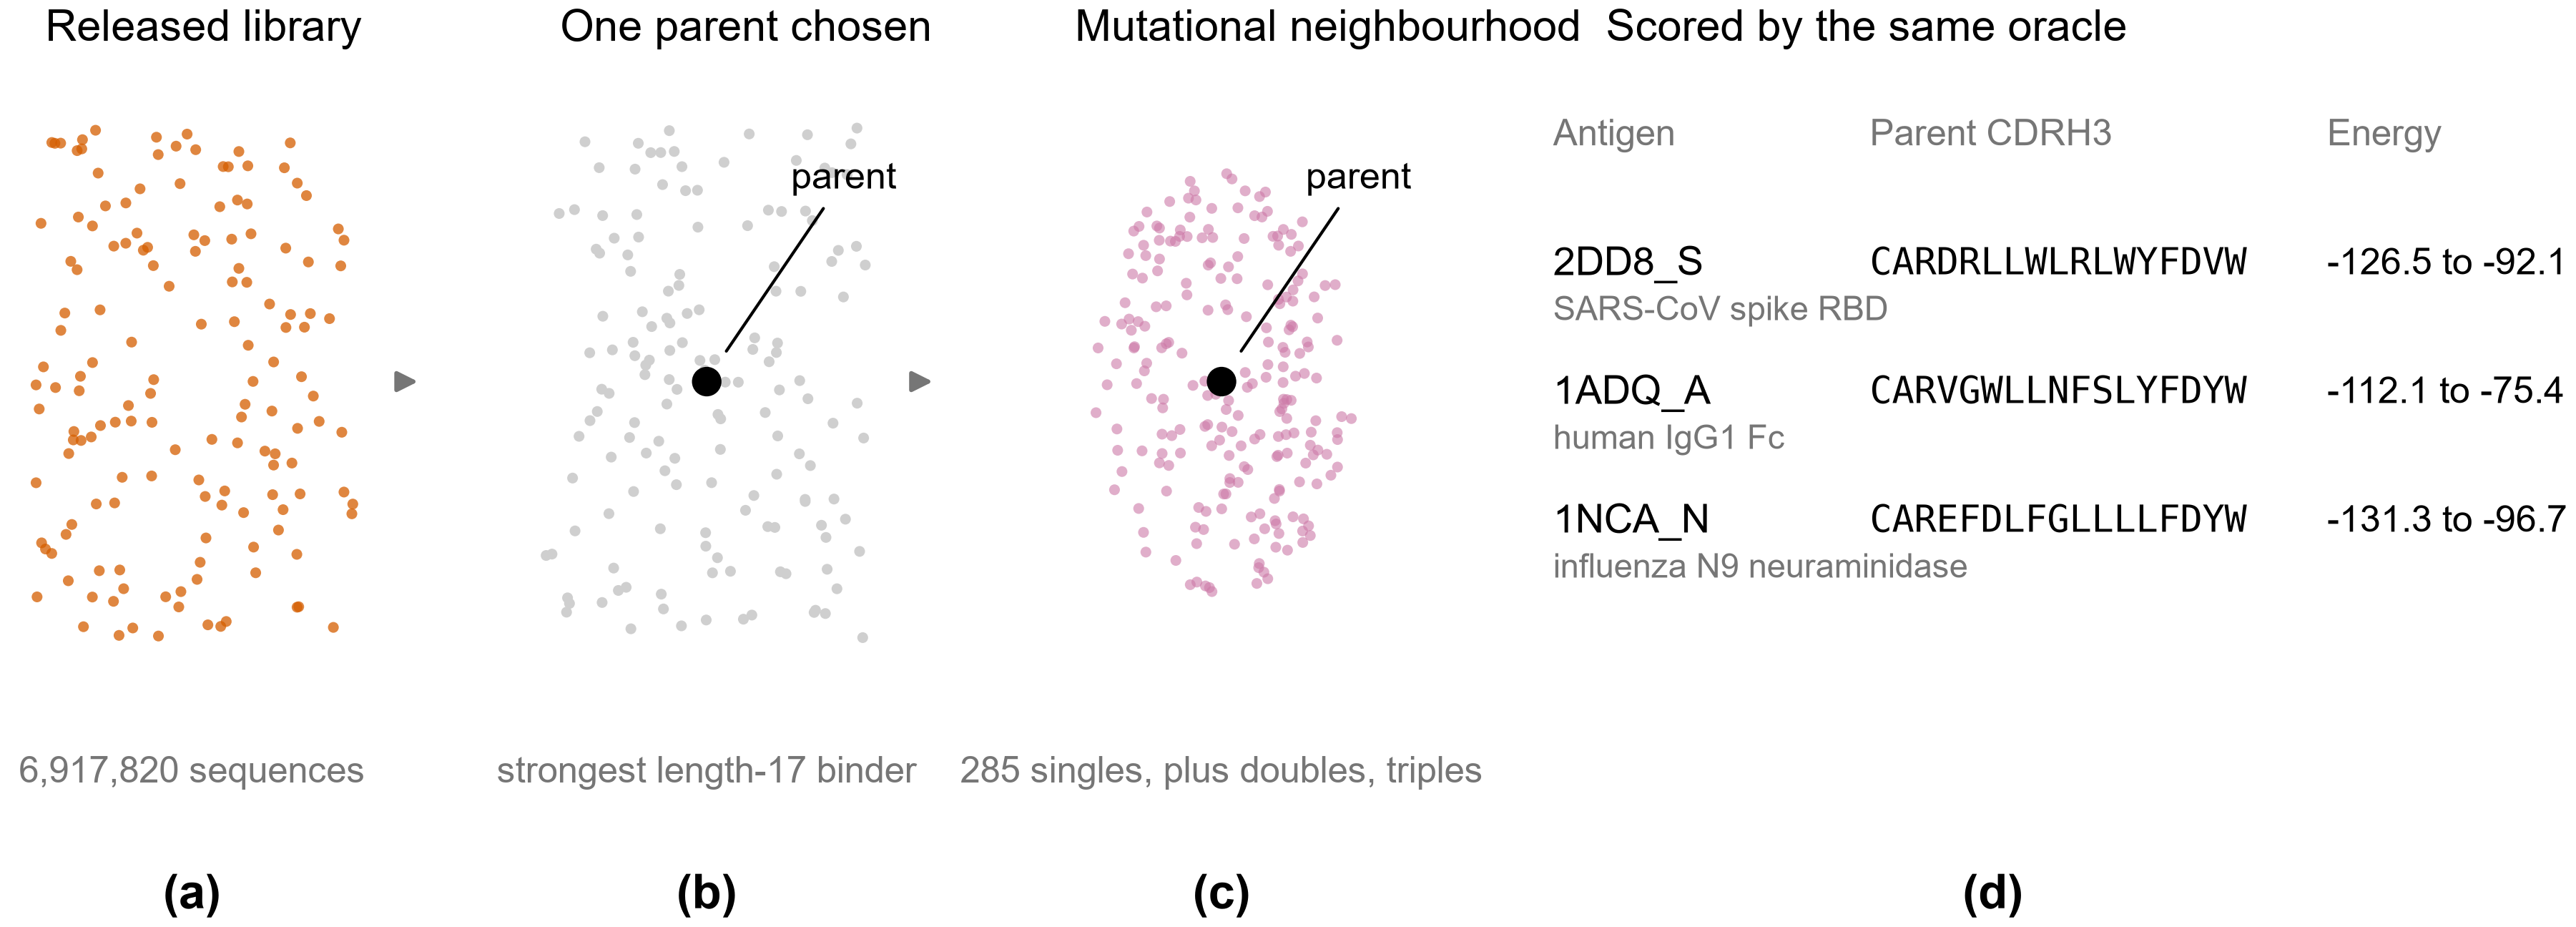
\includegraphics[width=\textwidth]{figs/F1.png}
\caption{Construction of the matched libraries. \textbf{(a)}, the released
library of unrelated CDRH3 sequences. \textbf{(b)}, one parent is chosen, a
strong binder of length 17. \textbf{(c)}, the parent is perturbed the way a
wet-lab library is perturbed, giving a mutational neighbourhood rather than a
sample. \textbf{(d)}, the seven libraries built this way, 6{,}000 sequences
each. Each has the size and the mutational structure of a measured dataset
while its labels still come from the lattice oracle; the Absolut! binary scores
every sequence, so the oracle, the antigen and the scoring function are
identical to those used for the released library, and the two dock into the
same pocket (Figure 2 of the main text).}\label{fig:matched}
\end{figure}

\begin{figure}[t]
\centering
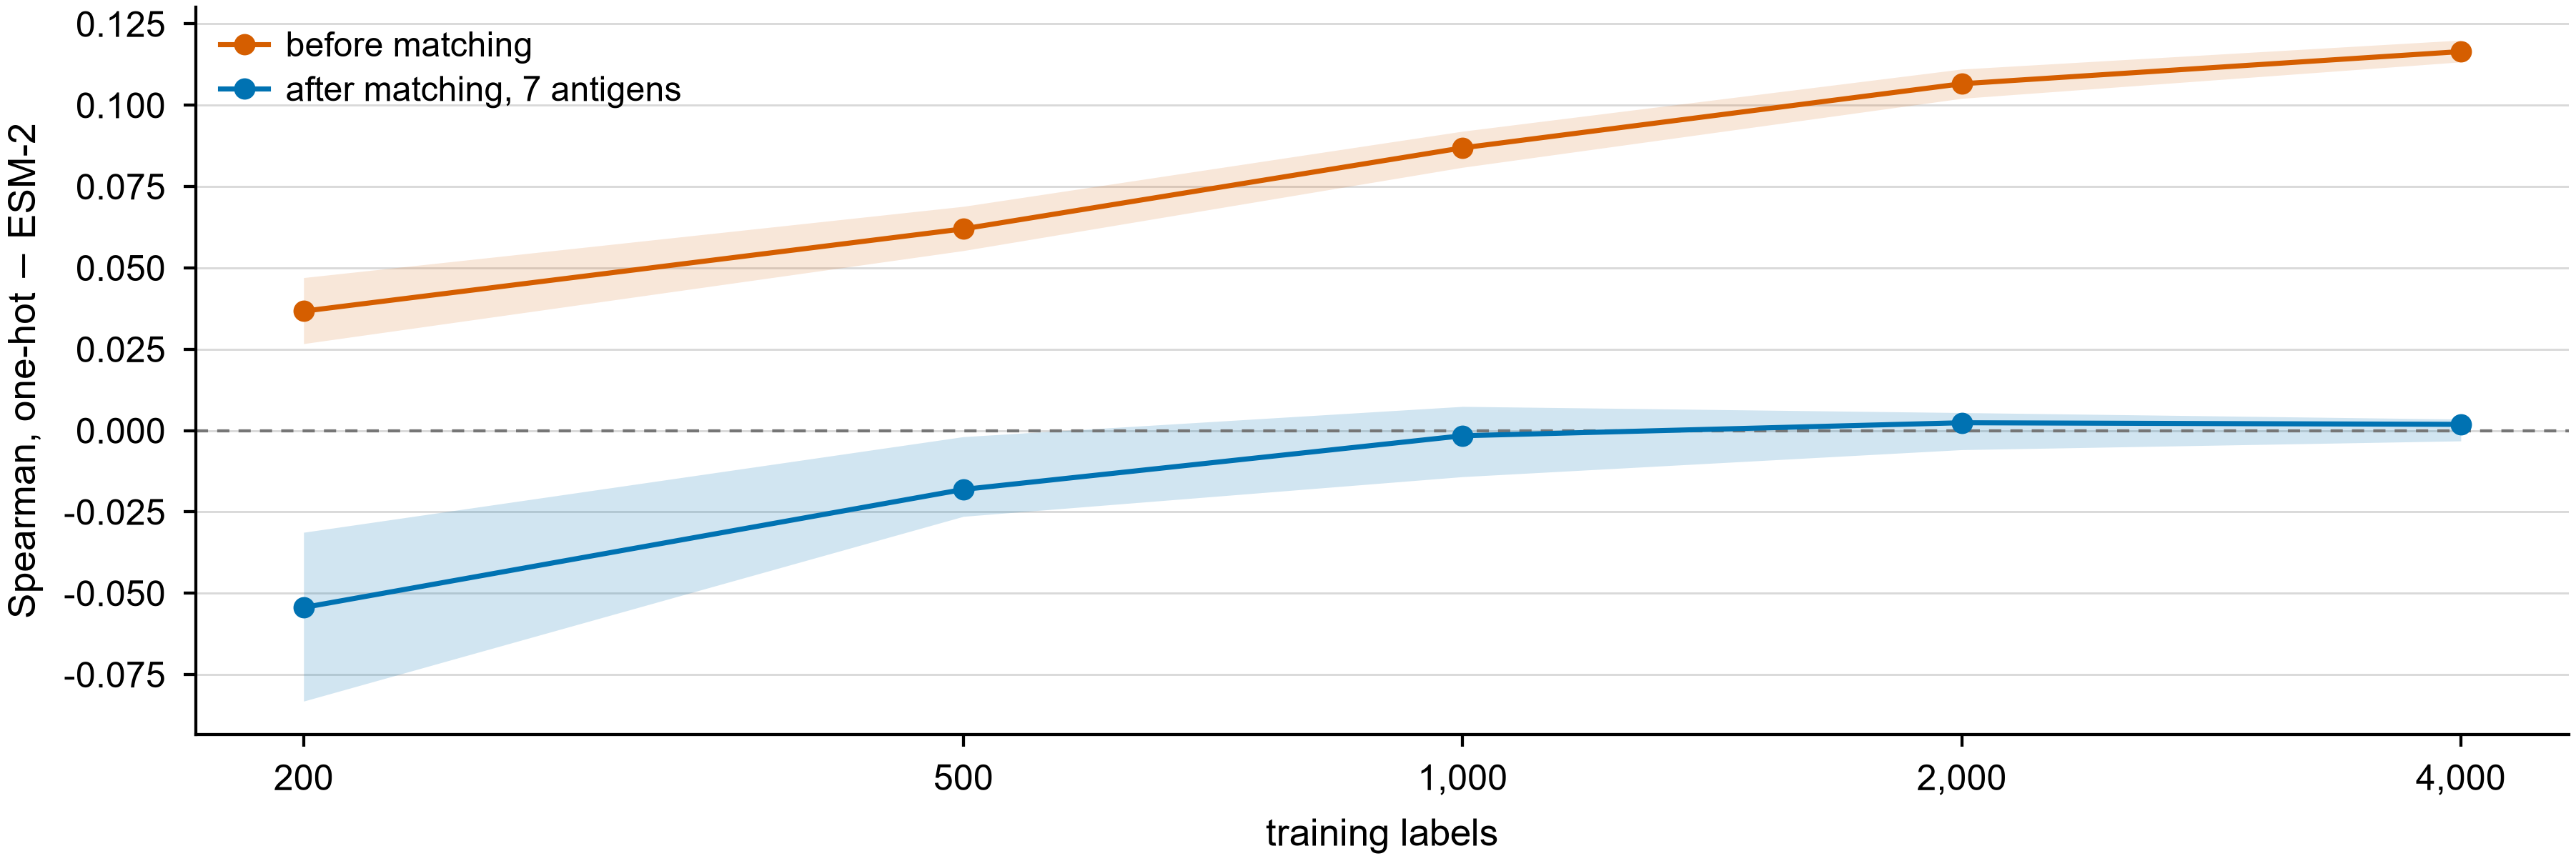
\includegraphics[width=\textwidth]{figs/F3.png}
\caption{Which representation is preferred depends on the label budget, and
matching reverses the direction of that dependence. The ordinate is the
difference in held-out Spearman between an aligned one-hot encoding and ESM-2
embeddings, so positive values favour one-hot. Before matching, on the released
library of 6.9 million unrelated sequences, one-hot is ahead at every budget and
its lead widens as labels accumulate; that band is a 95\% percentile bootstrap
interval over twenty splits. After matching, the language model is ahead at
small budgets and the advantage not only shrinks but reverses: the line is the
median over the seven matched libraries and the band their full range, and at
4{,}000 labels one-hot is ahead in five of the seven. Per-antigen values are in
Supplementary Table~S8. The same Absolut! oracle scores every library; only
their composition and, necessarily, the encoder differ.}\label{fig:structure}
\end{figure}

\begin{figure}[t]
\centering
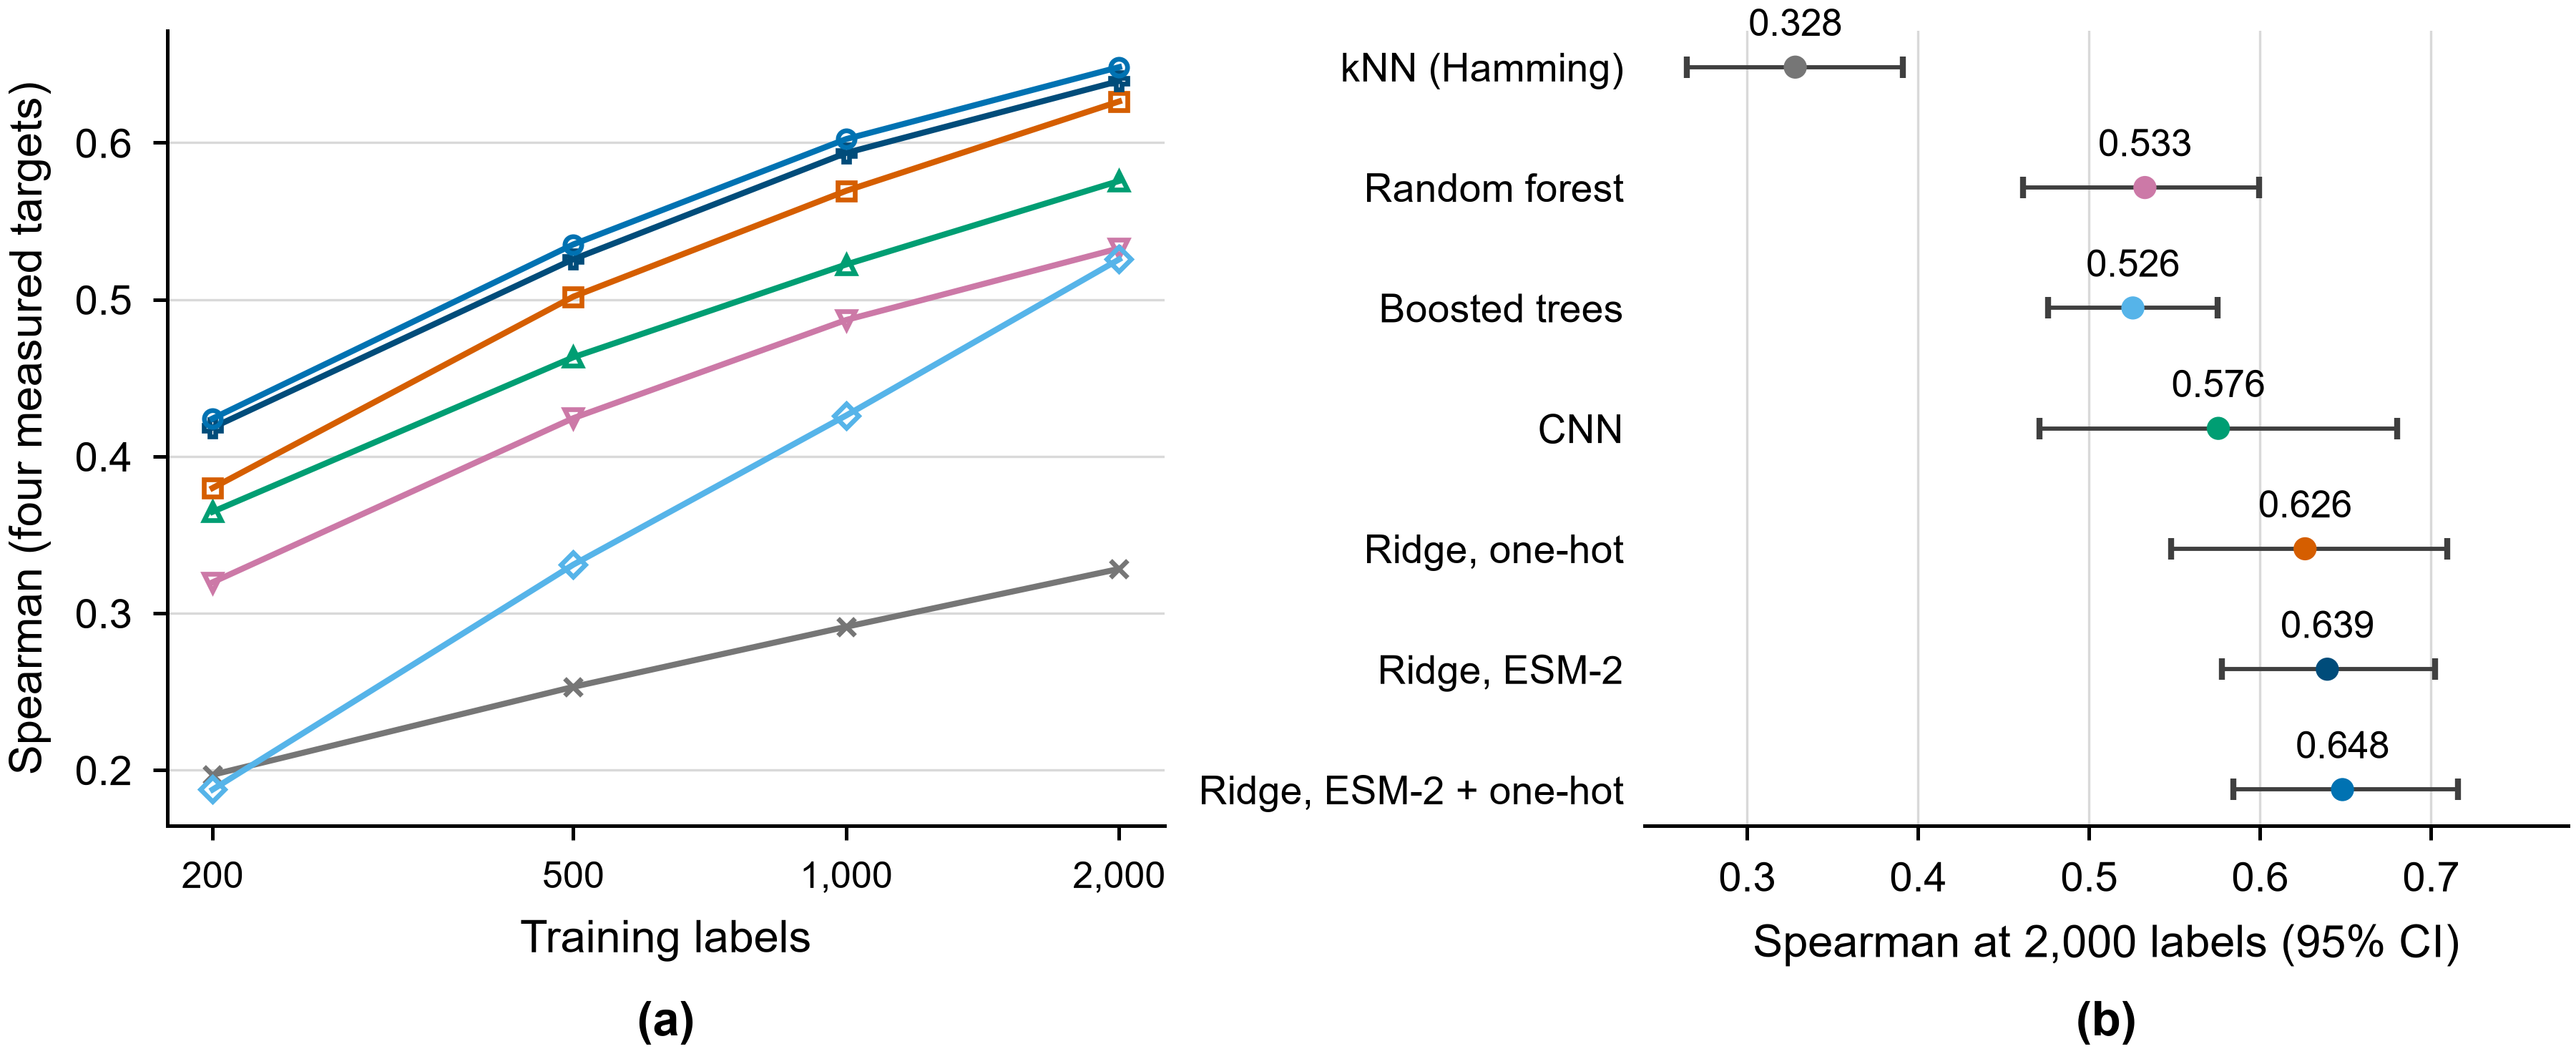
\includegraphics[width=\textwidth]{figs/F5.png}
\caption{Seven models across the four measured targets. Both panels are
restricted to training-set sizes at which all four targets are present, since
the available sizes differ between targets and averaging over the full range
would mix a trend with a change of composition. \textbf{(a)}, learning curves,
averaged over targets; each model keeps the colour it is given in \textbf{(b)},
which names them, so no key is repeated here. \textbf{(b)}, performance at
2{,}000 training labels with
95\% intervals from a bootstrap that resamples targets rather than predictions,
since nested subsets of one dataset are not independent observations. The
nearest-neighbour control separates clearly from the remaining models, which is
the minimal evidence that the comparison is not dominated by dataset
structure.}\label{fig:zoo}
\end{figure}

\vspace{1em}
\noindent Supplementary Data accompany this document as a separate archive. It
contains the per-experiment result tables from which every figure and every
quantity in the article is computed, and a file mapping each reported number
to the table and computation that produced it. The matched libraries are not
included; their specifications and sha256 digests are, with the script that
rebuilds them from a reader's own licensed Absolut! download.

\clearpage

\section*{Additional analyses not used for the primary conclusions}

Additional analyses that are not used for the primary conclusions. They bear on how far the matched construction generalises and are reported for completeness; no claim in the article rests on them.

\subsection*{What the lattice oracle does not encode}

The results above concern whether a method ranking transfers, not whether
lattice energies track real binding; a benchmark can order methods faithfully
while its labels are not a model of the biology. We tested the second question
using the benchmark's own provenance. Every Absolut! antigen comes from a
solved antibody--antigen complex, so each arrives with a cognate antibody,
whose CDRH3 we extracted and scored with the same oracle, asking whether the
oracle places a known binder above sequences not known to bind that antigen.

Of the 103 antigens, 88 support the test; the exclusions are itemised in
Supplementary Table~S6. For each we read the energy percentile of its cognate
CDRH3 against the full published table of 6.9 million sequences. The median was
44.2\%, and the distribution was indistinguishable from uniform
(Fig.~\ref{fig:scope}a; Kolmogorov--Smirnov $p = 0.78$, sign test $p = 0.34$).
It is unchanged when repeated sequences or structures are collapsed to one row
each ($p = 0.90$ and $0.91$) and on the 43 antigens whose cognate antibody is
murine like the comparison library (42.8\%, $p = 0.90$).

Because a single distribution is a weak test, we also scored each cognate CDRH3
against every other antigen and asked where its own antigen fell among the
rest. If the energy carried pairing information, the cognate antigen would rank
early. Its median rank was 0.484 of the way through, again indistinguishable
from uniform (Fig.~\ref{fig:scope}b; $p = 0.55$ over 90 antibodies). That
comparison is made within each antibody, so its length and composition cancel.

\begin{figure}[htbp]
\centering
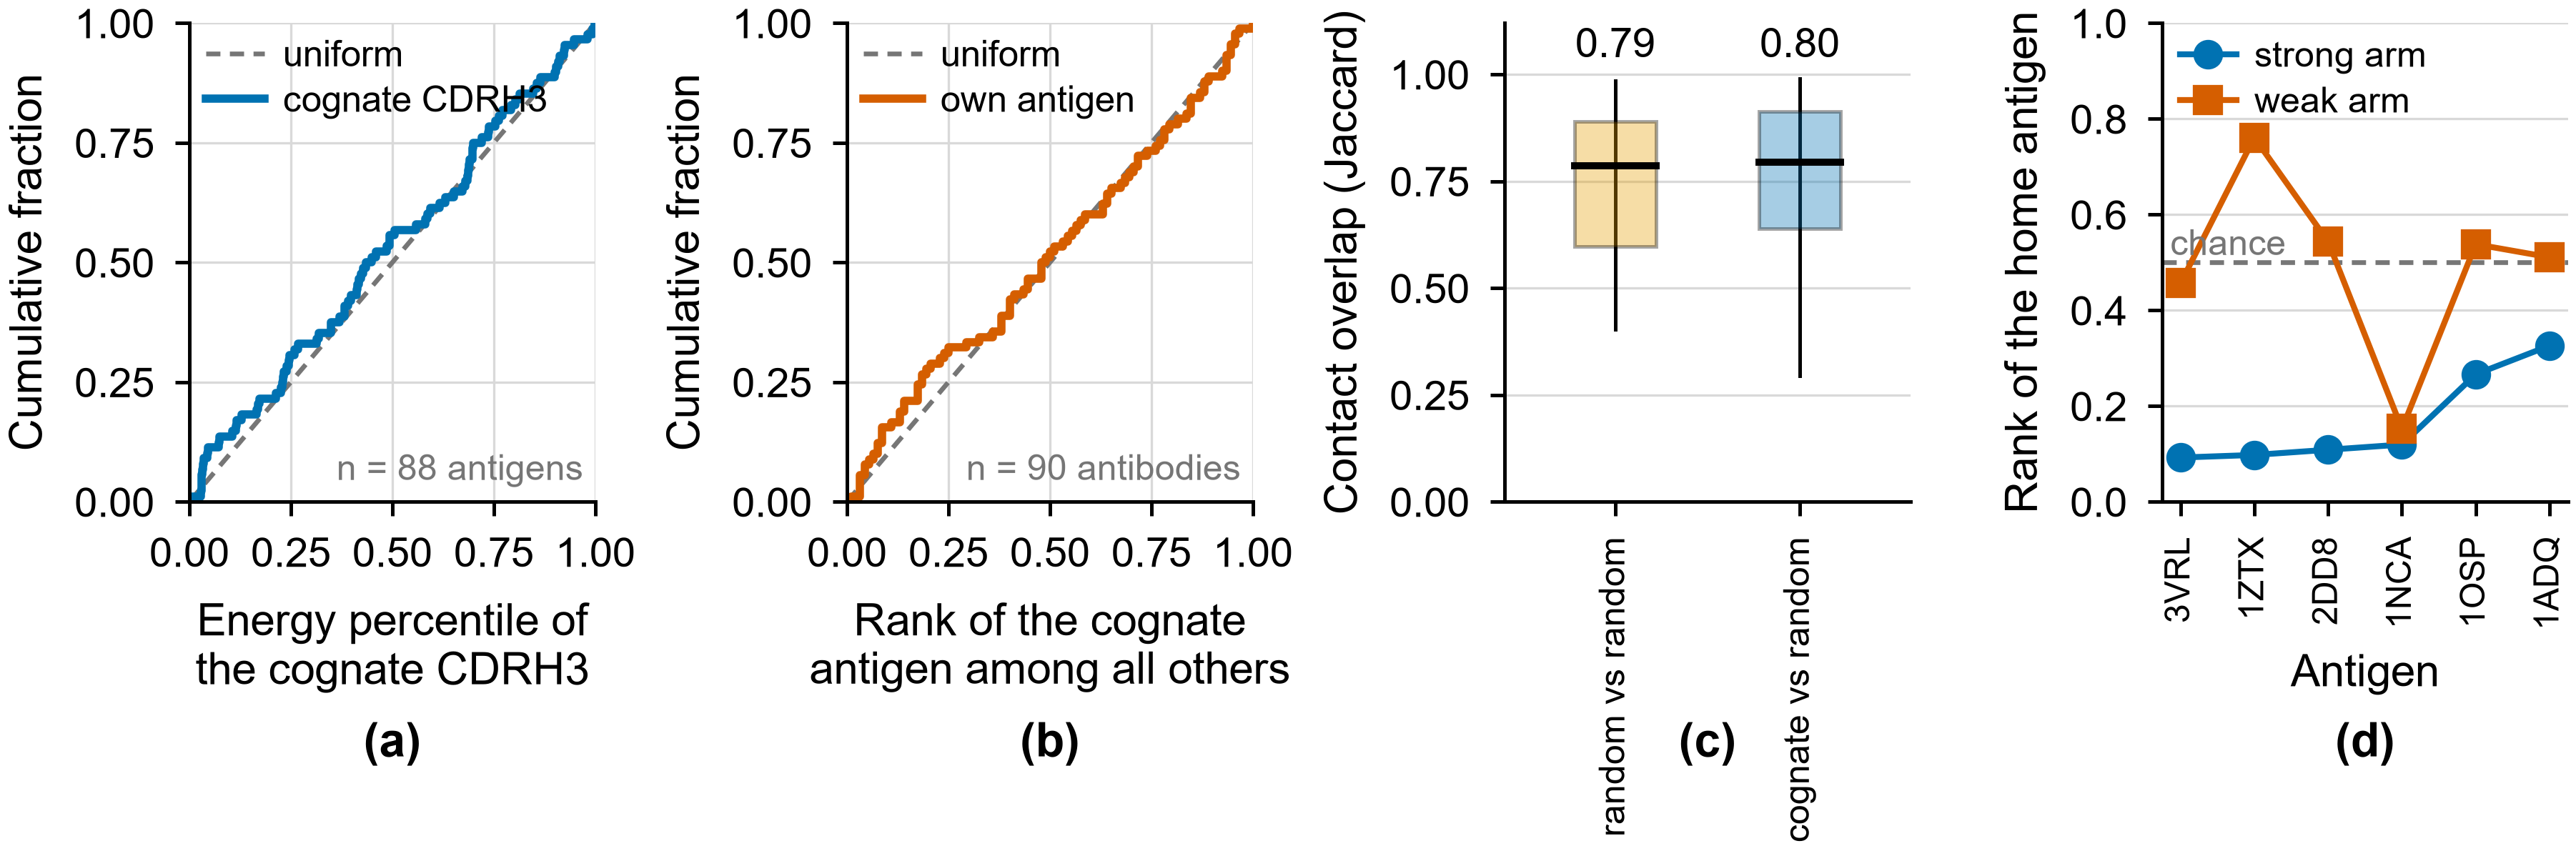
\includegraphics[width=\textwidth]{figs/F7.png}
\caption{What the lattice oracle does not encode. \textbf{(a)}, the energy
percentile of each antigen's cognate CDRH3 against the published library of
6.9 million sequences, as a cumulative distribution against the uniform
expectation. \textbf{(b)}, the same antibodies scored against every antigen:
the rank of the cognate antigen among all others. \textbf{(c)}, the reason.
Decoding the lattice pose gives the antigen residues each sequence contacts;
unrelated random sequences overlap each other as much as the cognate antibody
overlaps them, so the contact site is a property of the antigen rather than of
the sequence. Boxes are quartiles with the median marked and whiskers at the
5th and 95th percentiles. \textbf{(d)}, what the test can resolve, as a
function of binding strength. For each of six antigens, two arms share the
antigen, the CDRH3 length and the neighbourhood structure and differ only in
strength: a strong arm from the matched library, whose members the oracle
ranks in its top percentile, and a weak arm from the neighbourhood of a parent
at the 45th energy percentile, where the native cognate antibodies sit. The
strong arms place the home antigen consistently ahead of chance; the weak arms
largely do not, so the flat distributions in \textbf{(a)} and \textbf{(b)}
report a limit of the oracle in the range the native antibodies occupy rather
than a limit of the test. Tables~S18 and~S19 give the
intervals.}\label{fig:scope}
\end{figure}

The reason is visible in the poses. Absolut! records the position and move
string of the best-scoring pose and stores the antigen in the same encoding, so
the two can be laid on one lattice and the contacted residues read off. For the
cognate antibody and 200 random library sequences per antigen the contact site
barely moves: random sequences overlap one another with a median Jaccard of
0.79 and the cognate antibody overlaps them by 0.80 (Fig.~\ref{fig:scope}c),
with a median of 26 of 180 antigen residues contacted at all. The site is set
by the shape of the discretised antigen rather than by the sequence, which is
why the energies cannot separate cognate from non-cognate pairs. Consistent with this, in 32 of 90 antigens the
preferred site does not overlap the crystallographic epitope, and cognate and
random sequences are equally far from it (sign test $p = 0.91$).

The same thing shows directly in the energies. Scoring the identical 6.9
million sequences against each of the six antigens with full tables gives
correlations of 0.53 to 0.88 between any two, and 0.41 to 0.86 within length 17
alone, so length is not what drives it (Supplementary Table~S15). Their top
1{,}000 binders overlap by a median of 121 sequences where independence
predicts 0.14, and one pair shares the same best length-17 binder of
748{,}021. Much of what the oracle measures is therefore whether a sequence
binds well at all rather than whether it binds this antigen, which is the
uniform cognate percentile seen from the other side. The benchmark's authors
noted the phenomenon qualitatively, reporting that ``very similar antibody
sequences recognized different antigens'' and, when assembling their multiclass
dataset, ``discarding 11-mers that bound multiple antigens'' (Robert et al., 2022).
Its classification tasks therefore rest on a subset with cross-binders removed,
while a user scoring arbitrary sequences sees the unfiltered behaviour
quantified here.

\subsection*{Cognate-antibody test: methods}

For each of the 103 antigens the source PDB entry was retrieved and the
antibody heavy chain identified by its framework-4 motif at the variable-domain
position, rather than by the chain annotation, which is transposed in two
entries. The CDRH3 was taken as the segment from the conserved cysteine to that
motif and converted to the convention the oracle expects. Antigens were
excluded when the cognate CDRH3 was shorter than the 11-residue scoring window,
when the benchmark's antigen sequence did not align to any chain of the named
entry, when no antibody chain in the entry contacts the antigen chain the
benchmark uses (checked at 4.5~\AA{} between heavy atoms), or when a transfer,
archive or reproducibility gate failed; counts and reasons are in
Supplementary Table~S6. Percentiles count ties as half, because contact counts
are small integers and a strict comparison biases the cognate sequence upward.
Poses were decoded from the position and move string the binary reports; the
decoding was checked by requiring every antigen to fold without
self-intersection and to yield exactly as many residues as its stored sequence,
which 103 of 103 satisfy.

\subsection*{Model comparison and ranking transfer: methods}

Seven models were compared: ridge regression on aligned one-hot, on per-residue
ESM-2 embeddings and on both concatenated; a max-pooling convolutional network
over position tokens; a random forest; gradient-boosted trees; and a
ten-neighbour Hamming nearest-neighbour regressor, included as the control that
asks whether anything is being learned beyond proximity to a training sequence.
Every model sees the same split and the representation it requires. The
definitions live in one module imported by both the measured-target and the
lattice runs, so that a hyperparameter cannot drift between the arms while the
text calls them the same seven models.

For ranking transfer the models were ordered within each arm by mean held-out
Spearman at each training size, and the two orderings compared by Spearman
correlation. Confidence intervals come from resampling the seven antigens and
the four targets separately with replacement, 10{,}000 times, because those are
the two sources of variation in the means being ranked. Comparison is limited
to training sizes present in both arms, which the 6{,}000-sequence matched
libraries cap at 2{,}000.

\subsection*{Where the compared libraries sit among 217 public assays}

Those five properties are the ones we will hold fixed or vary deliberately, so
they need to be measurable rather than asserted. We implemented them as a tool,
\texttt{libmatch}, which reads two sequence--label tables and reports which of
the five differ and by how much (Methods). It takes any table with a sequence
column and a label column, so it is not tied to this benchmark. Figure~\ref{fig:axes}c
gives its output for four pairs, ordered by distance from the data it was
built on, and the dimension axis is mismatched in all four.

Measuring our own pair is a single comparison. To see whether that pair is
representative we ran the same tool over the 217 substitution assays of
ProteinGym (Notin et al., 2023), a collection of measured deep mutational scans
containing no antibody data (Fig.~\ref{fig:axes}). Every assay was read as a
mutational neighbourhood and every one was alignable, so neither structure nor
alignability separates them from the matched library. Size and training budget
do not single it out either: at 6{,}000 sequences it sits at the 72nd
percentile of the 217.

The number of varying positions does. The matched library varies 15 positions,
fewer than 96\% of the assays, with only 9 of 217 at or below it, while the
measured antibody data vary 89, at the 49th percentile. On the axis that this
paper will identify as the correlate of what survives matching, the measured
arm is typical of public measured data and the synthetic arm is extreme.

Profiling a collection once also lets the question be turned around: given a
dataset one intends to deploy on, which public datasets could be compared
against it without confounding? Asked of the matched library, 211 of the 217
assays differ on dimension while none differs on structure or noise, so almost
the whole benchmark is unusable as a comparator for it on the one axis that
matters here. Asked of the measured antibody data the picture is different:
161 differ on dimension, and the closest assay agrees on four of the five axes,
differing only in noise, which no released ProteinGym file can supply.

The noise axis cannot be compared at all. None of the 217 assays retains
replicate measurements, so for any of them the released file alone cannot say
how much of the label spread is measurement error. That is a property of how
such data are distributed rather than of how they were collected, and it bounds
what any comparison drawn from released files can establish.

\begin{figure}[htbp]
\centering
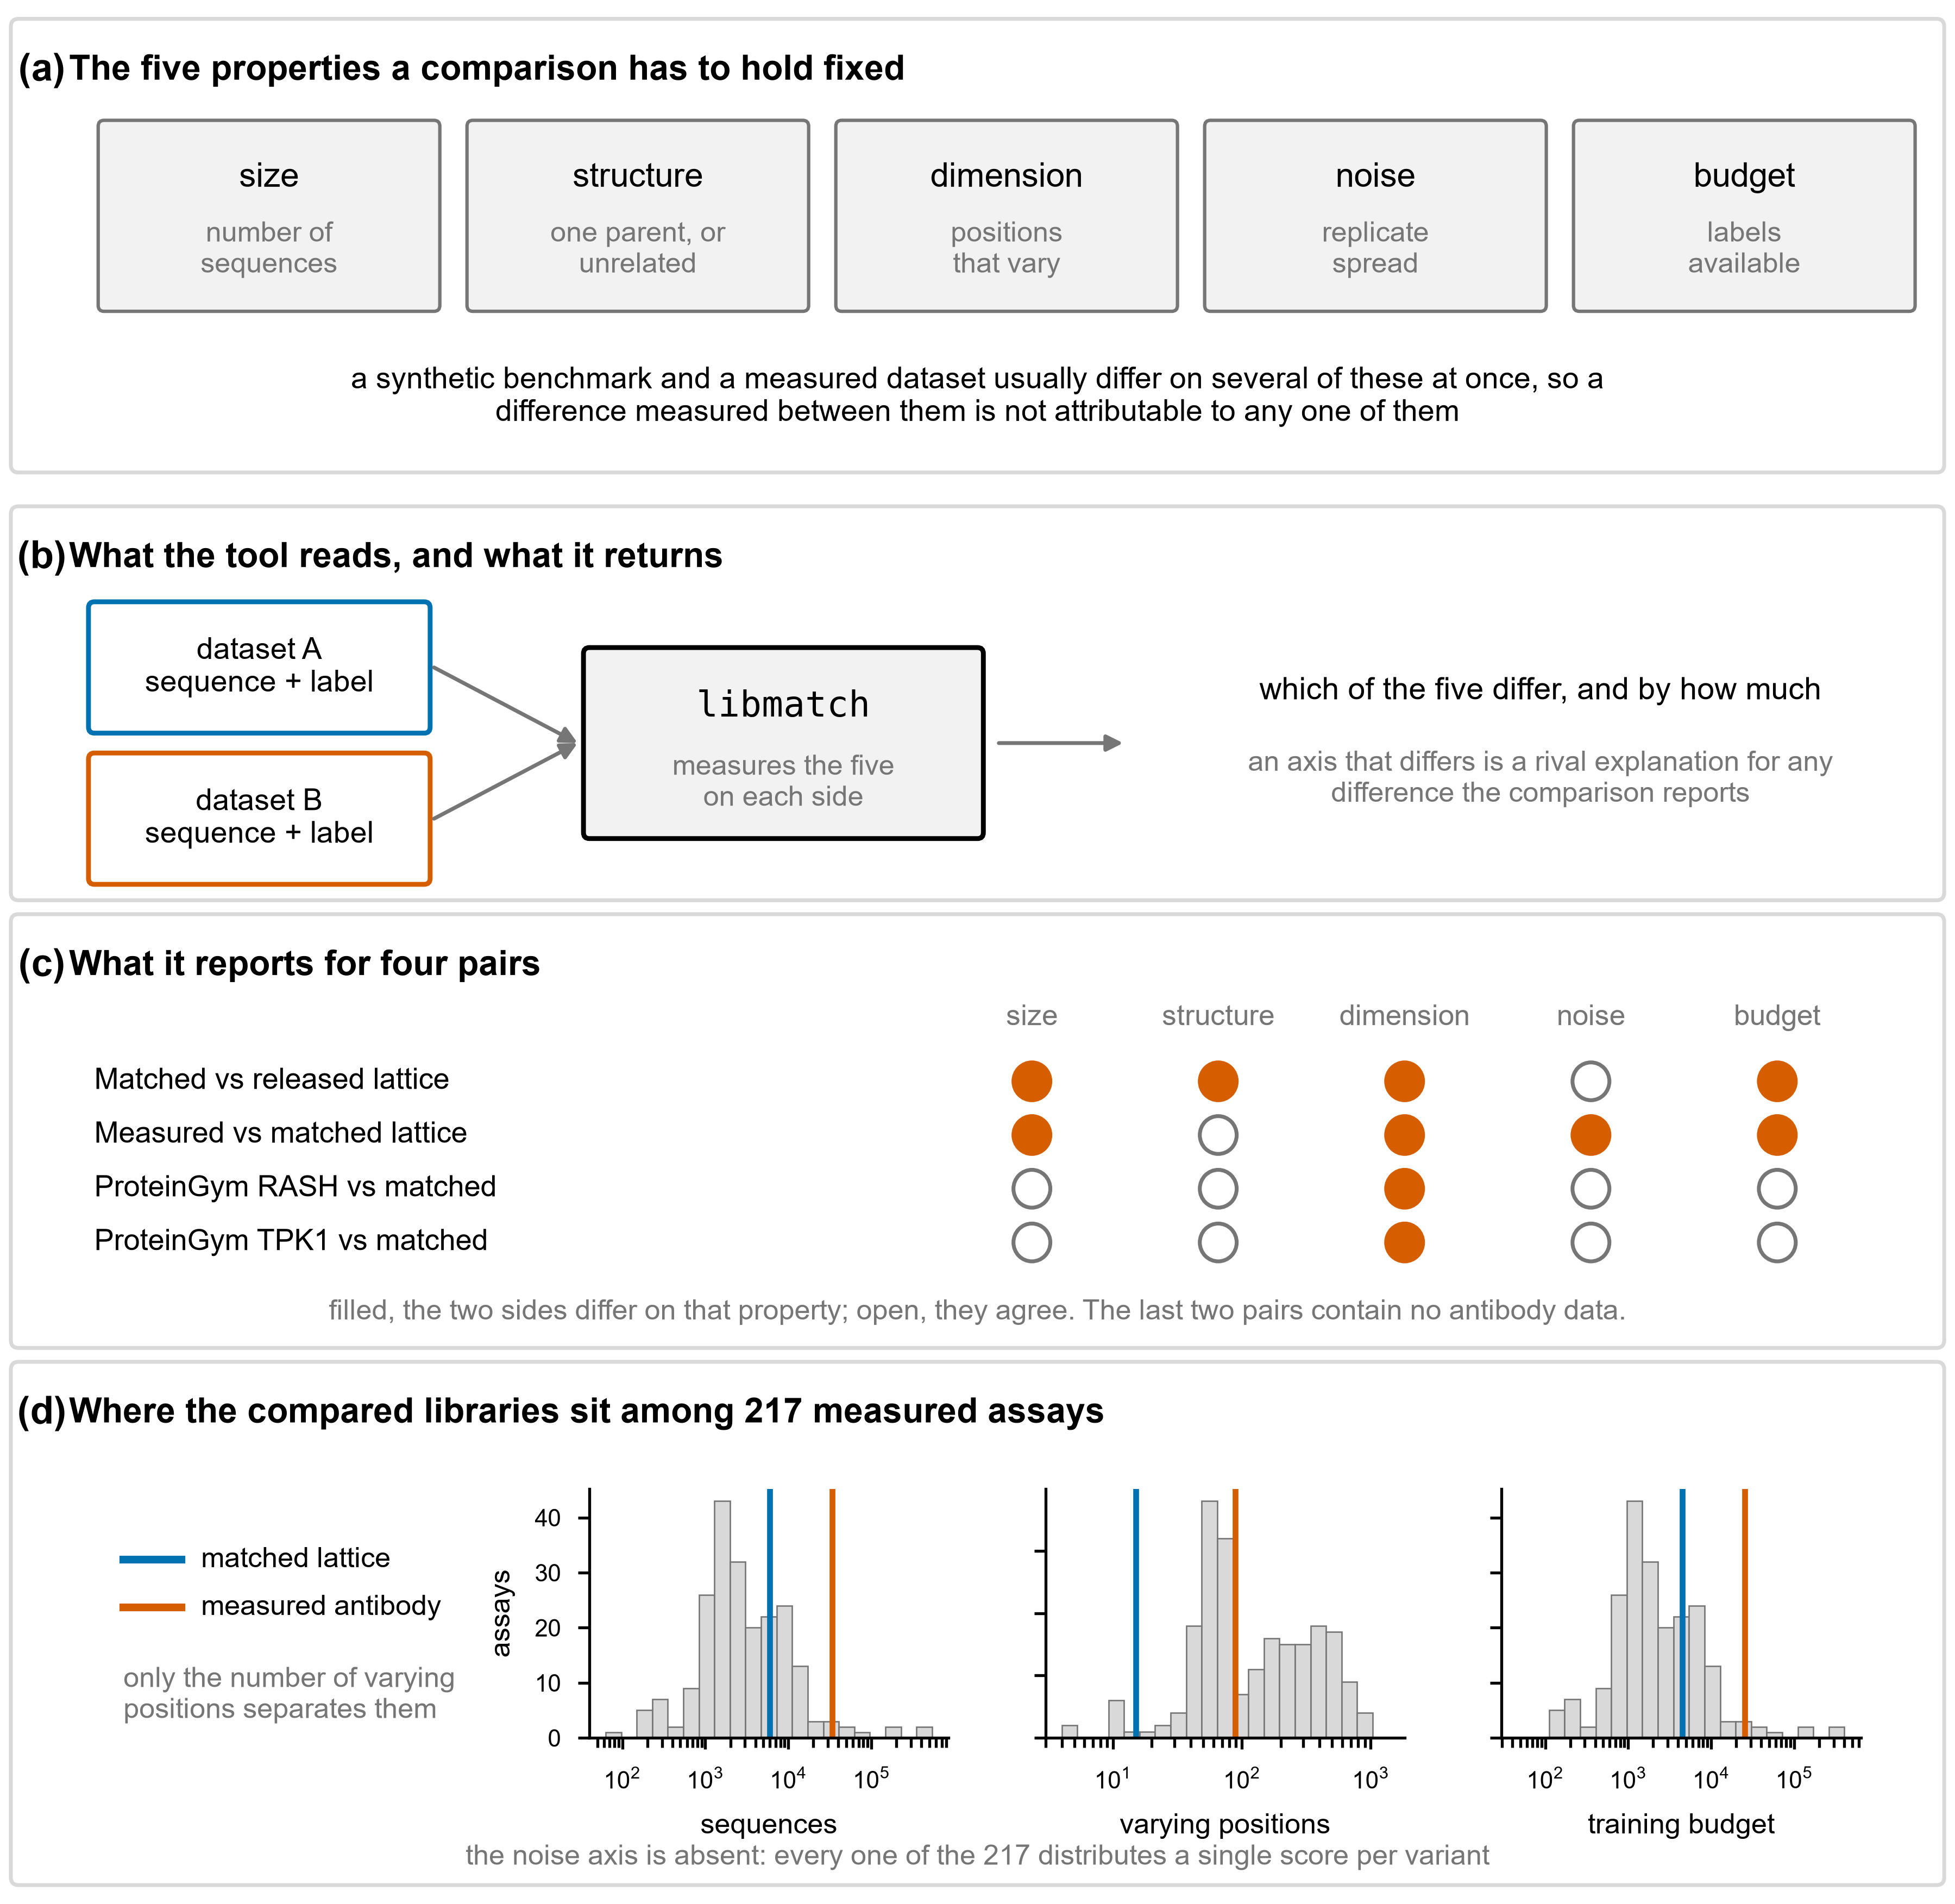
\includegraphics[width=\textwidth]{figs/F0.png}
\caption{What separates a benchmark from the data it stands in for.
\textbf{(a)}, the five operational axes the tool measures. A synthetic
benchmark and a measured dataset usually differ on several at once, which is
what makes a difference measured between them unattributable to any one of
them. These operational axes are distinct from the five dataset attributes in
Figure~1 of the main text; in particular, dimension and budget operationalise
alignability and evaluability, while label source is a property of how a
dataset was made rather than one countable from the file it is released as. \textbf{(b)}, the
tool reads two tables of sequences and labels and reports which of the five
differ and by how much; an axis that differs is a rival explanation for
whatever the comparison finds. \textbf{(c)}, its verdict for four pairs,
ordered by distance from the data it was built on. A filled circle marks an
axis the two sides differ on, an open circle one they share, and a dashed
circle one the tool could not measure on those two datasets. The third is not
the second: an axis that was never measured is not an axis that agrees, and
reporting it as agreement would turn a question that was not asked into a
finding. The last two pairs are deep mutational scans of non-antibody
proteins, distributed as mutation notation and expanded against the wild type;
the dimension axis is mismatched in all four, and the noise axis is measurable
in neither. A lattice energy is computed, so repeating it returns the same
value and its replicate spread is zero; a measured assay released with one
score per variant is indistinguishable from that in the file, but its spread
was averaged away before release. The tool is therefore told which kind of
label it is reading, and reports the axis as not measured where it is not
told. \textbf{(d)},
the same properties measured over the 217 substitution assays of ProteinGym,
with the two libraries compared here marked. Sizes and budgets place the
matched library near the middle of that distribution and only the number of
varying positions separates it, at the 4th percentile against the 49th for the
measured antibody data. The noise axis cannot be compared at all, because every
one of the 217 distributes a single score per variant.}
\label{fig:axes}
\end{figure}

\subsection*{Whether the benchmark ranks methods as measured data do}

\begin{figure}[htbp]
\centering
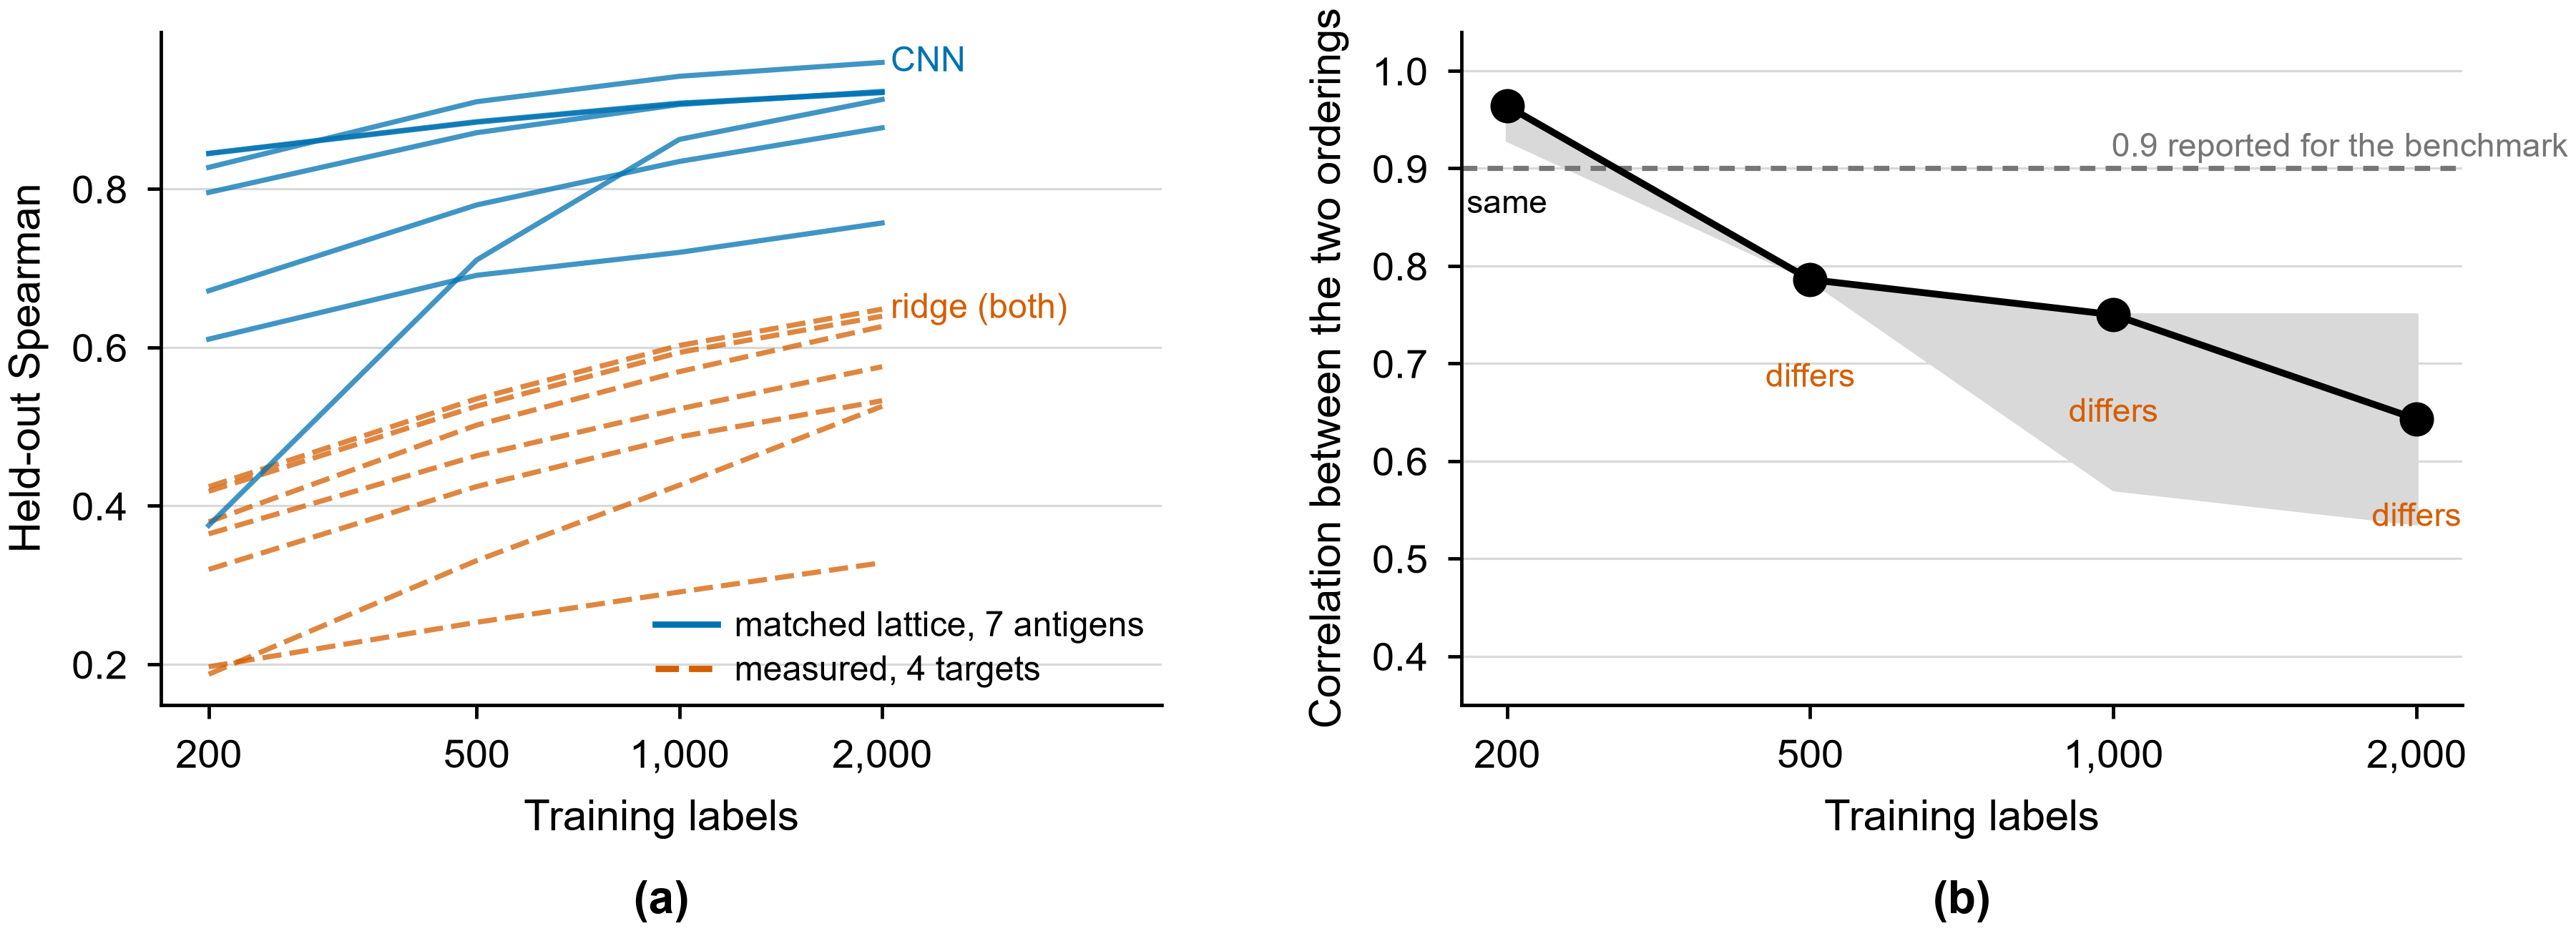
\includegraphics[width=\textwidth]{figs/F10.png}
\caption{Whether the benchmark ranks methods as the measured data do.
\textbf{(a)}, each of seven models against training size, solid on the seven
matched lattice libraries and dashed on the four measured targets, with only
the model leading each arm at the largest common budget named. The models are
fitted from one shared definition, so no hyperparameter differs between the
arms. \textbf{(b)}, the correlation between the two orderings at each budget,
with an interval from resampling antigens and targets separately; the label
below each point says whether the two arms put the same model first. Agreement
is high where labels are scarce and falls as they become plentiful, crossing
from the same leading model to a different one between 200 and 500 labels. The
dashed line is the correlation of 0.9 the benchmark's own validation reported
for method accuracies, obtained for one binary classification task with
classical classifiers; the budget at which our figure matches it is the
smallest one tested.}
\label{fig:transfer}
\end{figure}

What a benchmark is for is ranking methods, so we tested that directly rather
than through two representations. The seven models already fitted to the four
measured targets---ridge on one-hot, on language-model embeddings and on both,
a max-pooling convolutional network, random forest, gradient-boosted trees and
a nearest-neighbour control---were fitted to the seven matched lattice
libraries from a single shared definition, so no hyperparameter can differ
between the arms. At each training size the models were ordered within each arm
by mean held-out Spearman and the two orderings compared, with intervals from
resampling antigens and targets separately.

Agreement depends on the budget. At 200 labels the orderings correlate at
$+0.964$ (95\% CI $+0.929$ to $+0.964$) and both arms rank the same model
first. The correlation then falls monotonically, to $+0.786$ at 500, $+0.750$
at 1{,}000 and $+0.643$ ($+0.536$ to $+0.750$) at 2{,}000, and from 500 labels
upwards the best model on the lattice is no longer the best on measured data:
the convolutional network wins on the lattice while the combined-representation
ridge wins on measured targets (Fig.~\ref{fig:transfer}; Supplementary Table~S20).

This locates rather than contradicts the benchmark's own validation. Its
authors reported a correlation of 0.9 between method accuracies on the
benchmark and on a measured dataset (Robert et al., 2022), obtained for one binary
classification task with classical classifiers; our figure at the smallest
budget agrees with theirs. What the larger budgets add is that the agreement is
not a fixed property of the benchmark. It is strongest where a model has too
few labels to exploit the structure that distinguishes the two libraries, and
it decays as that structure becomes learnable---the same budget dependence the
representation comparison shows, measured on model architecture instead.

% ---- BEGIN supplementary methods (generated)
\clearpage

\section*{Supplementary Methods}

\subsection*{Encoders}

The two arms of the representation comparison cannot share an encoder. In a
matched library every sequence is a variant of one parent and has the same
length, so position $i$ of one sequence corresponds to position $i$ of another
and an aligned one-hot encoding is defined: 21 indicator columns per varying
position. The released library is 6{,}917{,}820 unrelated CDRH3 sequences of
lengths 11 to 43, where no such correspondence exists. There a sequence is
encoded by positional one-hot over the 11 residues at each terminus, counts of
all 400 dipeptides, and a one-hot of the length. ESM-2 features are computed
the same way in both arms -- per-residue embeddings from layer 12 of the
35M-parameter checkpoint, reduced to 48 principal components fitted on a sample
of residue vectors -- but at different positions, because the arms have
different notions of position: the positions that vary within a matched
library, and the first 26 positions of the released one. Ridge regularisation is $\alpha = 1$ for one-hot and $\alpha = 50$ for
the embeddings, values fixed before the comparisons reported here and unchanged
between arms.

\subsection*{Noise injection}

Measurement noise was estimated from 100 replicate AlphaSeq measurements of the
wild-type parent in each campaign ($\sigma = 0.27$ in $\log_{10} K_D$), giving
a mean noise-to-signal ratio of 0.424 across the four targets. Gaussian noise
at that ratio of the label standard deviation was added to matched lattice
labels.

\subsection*{Prospective evaluation}

The AlphaSeq coronavirus panel contains two design campaigns. The retrospective
task splits one campaign at random; the prospective task trains on the first
campaign and tests on the second, after removing from the test set every
sequence that also appears in the first, so that re-measured designs cannot
inflate the result. To characterise the shift between campaigns we encoded both
sets one-hot against the most frequent sequence and took the first two
components of a truncated singular value decomposition, and separately counted
the number of substitutions of each sequence from that reference. Batch effects
were assessed using the wild-type replicates present in both campaigns.

\subsection*{Panning re-analysis}

Clonotype abundances were computed per round after rarefying every library to
the smallest sequencing depth in the series and discarding clonotypes seen
fewer than five times, since diversity statistics and enrichment ratios are
both sensitive to depth. Three tasks were compared for identifying the top 1\%
of final-round clonotypes: a random forest on early-round read counts; a
baseline that ranks by the last available early round alone; and a model given
only the CDR3 sequence, with no abundance information. A permutation null was
obtained by shuffling labels over twenty repetitions.

\subsection*{Software and reproducibility}

Analyses were run in Python with scikit-learn, PyTorch, pandas and SciPy; ESM-2
embeddings were computed with the released 35M-parameter checkpoint. The
Absolut! binary was built from its public repository under Linux; on Windows it
linked but crashed while reading structure files, so all scoring was performed
under Linux. Each experiment writes one result table, provided as Supplementary
Data and named after the experiment that produced it, and every quantity in the
text and in the supplementary tables is computed from those tables by the
scripts that generate the tables and figures.
% ---- END supplementary methods

% ---- BEGIN cognate disposition (generated)
\begin{table}[h]
\caption{Disposition of the 103 Absolut! antigens in the cognate-antibody test. Exclusions are listed with their reason so that the denominator can be checked; none of the classes is defined by the outcome of the test.}
\centering
\begin{tabular}{@{}p{7.4cm}rp{4.4cm}@{}}
\toprule
Disposition & $n$ & Reason \\
\midrule
Scored, full published table & 88 & used in the main analysis \\
Scored, published table covers 97.5--97.6\% of the library (3RVV\_A, 3SKJ\_E) & 2 & reported separately with exact bounds \\
Cognate CDRH3 shorter than the 11-residue scoring window (1NSN\_S, 2Q8A\_A, 2R4R\_A, 2UZI\_R, \ldots) & 6 & the oracle returns no value \\
Antibody in the source entry does not contact the antigen chain (4K24\_A, 4K3J\_A) & 2 & the pair is not a binder of this antigen \\
Antigen sequence absent from the named PDB entry (3L5W\_I) & 1 & provenance cannot be established \\
Two distinct antibodies bound to the same antigen & 2 & no single cognate CDRH3 \\
Conserved cysteine absent from the heavy chain & 1 & not expressible in the oracle's convention \\
Published table archive corrupt at source (4N9G\_C) & 1 & size and checksum match the server, but the archive is truncated \\
\midrule
Total & 103 & \\
\bottomrule
\end{tabular}
\end{table}
% ---- END cognate disposition
% ---- BEGIN unmatched seeds (generated)
\begin{table}[h]
\caption{The unmatched arm of the representation comparison, measured with the protocol used for the matched arm: twenty independent train/test splits, the same training sizes, the same models and the same seeds. Positive values favour one-hot. The advantage is present at every size and widens with training data, so the effect that matching removes is not an artefact of the three to five splits used in the first pass.}
\centering
\begin{tabular}{@{}rrrrrr@{}}
\toprule
Training labels & Splits & Mean & 95\% CI & one-hot wins & $p$ (paired $t$) \\
\midrule
200 & 20 & +0.0367 & +0.0267 to +0.0470 & 18/20 & 1.6e-06 \\
500 & 20 & +0.0620 & +0.0553 to +0.0689 & 20/20 & 5.4e-13 \\
1,000 & 20 & +0.0869 & +0.0809 to +0.0920 & 20/20 & 2.4e-17 \\
2,000 & 20 & +0.1066 & +0.1021 to +0.1111 & 20/20 & 8.8e-21 \\
4,000 & 20 & +0.1165 & +0.1133 to +0.1200 & 20/20 & 5.6e-24 \\
\midrule
Pooled & 100 cells & +0.0817 & & 98/100 & \\
\bottomrule
\end{tabular}
\end{table}
% ---- END unmatched seeds
% ---- BEGIN repr many antigens (generated)
\begin{table}[h]
\caption{The representation comparison on every matched library that passed the consistency check, each measured with the protocol used for 2DD8\_S: twenty independent train/test splits, the same training sizes, the same two models and the same seeds. Only the antigen changes. Negative values favour the language model. The advantage is a function of the label budget rather than of the antigen: it is largest at 200 labels and decays monotonically, so the ordering of the two representations is not a fixed property of the matched library. Intervals exclude zero in favour of the language model for 5 of 5 antigens and in favour of one-hot for 0.}
\centering
\begin{tabular}{@{}lrrrrr@{}}
\toprule
Antigen & Labels & Mean & 95\% CI & ESM ahead & $p$ (paired $t$) \\
\midrule
1ADQ\_A & 200 & -0.0363 & -0.0414 to -0.0307 & 20/20 & 7.3e-11 \\
 & 500 & -0.0264 & -0.0285 to -0.0246 & 20/20 & 4.1e-16 \\
 & 1,000 & -0.0142 & -0.0165 to -0.0119 & 20/20 & 3.7e-10 \\
 & 2,000 & -0.0059 & -0.0069 to -0.0050 & 20/20 & 1.8e-10 \\
 & 4,000 & -0.0032 & -0.0037 to -0.0028 & 20/20 & 3.8e-11 \\
\textit{pooled} & 100 cells & -0.0172 & -0.0200 to -0.0145 & 100/100 & 1.9e-21 \\
\midrule
1NCA\_N & 200 & -0.0544 & -0.0591 to -0.0499 & 20/20 & 5.1e-15 \\
 & 500 & -0.0101 & -0.0131 to -0.0075 & 20/20 & 1.9e-06 \\
 & 1,000 & +0.0026 & +0.0014 to +0.0037 & 2/20 & 3.0e-04 \\
 & 2,000 & +0.0045 & +0.0038 to +0.0051 & 0/20 & 1.2e-10 \\
 & 4,000 & +0.0033 & +0.0028 to +0.0038 & 0/20 & 3.8e-11 \\
\textit{pooled} & 100 cells & -0.0108 & -0.0155 to -0.0064 & 42/100 & 1.0e-05 \\
\midrule
1OSP\_O & 200 & -0.0609 & -0.0656 to -0.0561 & 20/20 & 6.9e-16 \\
 & 500 & -0.0187 & -0.0222 to -0.0153 & 20/20 & 3.1e-09 \\
 & 1,000 & -0.0016 & -0.0034 to +0.0001 & 12/20 & 9.1e-02 \\
 & 2,000 & +0.0024 & +0.0014 to +0.0034 & 3/20 & 2.2e-04 \\
 & 4,000 & +0.0019 & +0.0014 to +0.0024 & 1/20 & 1.3e-06 \\
\textit{pooled} & 100 cells & -0.0154 & -0.0203 to -0.0106 & 56/100 & 1.5e-08 \\
\midrule
1ZTX\_E & 200 & -0.0557 & -0.0596 to -0.0516 & 20/20 & 1.6e-16 \\
 & 500 & -0.0019 & -0.0036 to -0.0002 & 15/20 & 4.2e-02 \\
 & 1,000 & +0.0074 & +0.0067 to +0.0080 & 0/20 & 7.5e-15 \\
 & 2,000 & +0.0055 & +0.0052 to +0.0058 & 0/20 & 1.2e-19 \\
 & 4,000 & +0.0035 & +0.0033 to +0.0037 & 0/20 & 4.4e-19 \\
\textit{pooled} & 100 cells & -0.0082 & -0.0132 to -0.0035 & 35/100 & 1.1e-03 \\
\midrule
2DD8\_S & 200 & -0.0365 & -0.0447 to -0.0284 & 20/20 & 5.6e-08 \\
 & 500 & -0.0181 & -0.0231 to -0.0126 & 19/20 & 2.3e-06 \\
 & 1,000 & -0.0071 & -0.0098 to -0.0043 & 18/20 & 7.7e-05 \\
 & 2,000 & -0.0009 & -0.0018 to +0.0001 & 13/20 & 8.4e-02 \\
 & 4,000 & +0.0000 & -0.0006 to +0.0007 & 10/20 & 9.2e-01 \\
\textit{pooled} & 100 cells & -0.0125 & -0.0160 to -0.0093 & 80/100 & 7.4e-11 \\
\bottomrule
\end{tabular}
\end{table}
% ---- END repr many antigens
% ---- BEGIN search ci (generated)
\begin{table}[h]
\caption{The search advantage measured with twenty seeds and a bootstrap interval on the reported quantity. Library, budgets, strategies, the top-1\% rule and the seed rule are those of the first pass; only the number of seeds and the reporting changed. The ratio is of mean recovery, so the interval resamples seeds and recomputes the ratio of means rather than averaging per-seed ratios, which are undefined whenever random search recovers nothing. At a budget of 200 the guided strategies spend the whole budget on their initial random sample and never fit a model, so a ratio of 1.00 there is a property of the design and not a result. Where active recovery reaches 1.000 the ratio is a lower bound rather than a value, because the top 1\% has been recovered in full and the numerator cannot rise further. At a budget of 1{,}000 the measured targets span 2.11 to 3.35-fold and the matched lattice 3.71 to 6.15; only the lowest matched library overlaps that range. Matching library size and mutational structure therefore narrows this difference by three orders of magnitude without closing it.}
\centering
\begin{tabular}{@{}lrrrrr@{}}
\toprule
Library & Budget & Active & Random & Ratio & 95\% CI \\
\midrule
1ADQ\_A (matched lattice) & 200 & 0.035 & 0.035 & 1.00 & 1.00 to 1.00 \\
1NCA\_N (matched lattice) & 200 & 0.036 & 0.036 & 1.00 & 1.00 to 1.00 \\
2DD8\_S (matched lattice) & 200 & 0.031 & 0.031 & 1.00 & 1.00 to 1.00 \\
1ADQ\_A (matched lattice) & 500 & 0.805 & 0.080 & 10.06 & 8.37 to 12.17 \\
1NCA\_N (matched lattice) & 500 & 0.944 & 0.090 & 10.49 & 8.81 to 12.76 \\
2DD8\_S (matched lattice) & 500 & 0.457 & 0.077 & 5.96 & 4.99 to 7.10 \\
1ADQ\_A (matched lattice) & 1,000 & 0.951 & 0.165 & 5.76 & 5.00 to 6.71 \\
1NCA\_N (matched lattice) & 1,000 & 1.000 & 0.163 & 6.15 & 5.36 to 7.27 \\
2DD8\_S (matched lattice) & 1,000 & 0.643 & 0.173 & 3.71 & 3.34 to 4.18 \\
\midrule
CoV2-RBD (measured) & 200 & 0.033 & 0.033 & 1.00 & 1.00 to 1.00 \\
HER2 (measured) & 200 & 0.045 & 0.045 & 1.00 & 1.00 to 1.00 \\
PD-1 (measured) & 200 & 0.034 & 0.034 & 1.00 & 1.00 to 1.00 \\
TIGIT (measured) & 200 & 0.027 & 0.027 & 1.00 & 1.00 to 1.00 \\
CoV2-RBD (measured) & 500 & 0.201 & 0.078 & 2.56 & 2.07 to 3.23 \\
HER2 (measured) & 500 & 0.326 & 0.090 & 3.62 & 2.83 to 4.72 \\
PD-1 (measured) & 500 & 0.174 & 0.087 & 1.99 & 1.57 to 2.58 \\
TIGIT (measured) & 500 & 0.288 & 0.080 & 3.60 & 3.11 to 4.25 \\
CoV2-RBD (measured) & 1,000 & 0.333 & 0.158 & 2.11 & 1.77 to 2.50 \\
HER2 (measured) & 1,000 & 0.578 & 0.172 & 3.35 & 2.92 to 3.86 \\
PD-1 (measured) & 1,000 & 0.347 & 0.162 & 2.14 & 1.81 to 2.54 \\
TIGIT (measured) & 1,000 & 0.459 & 0.171 & 2.69 & 2.40 to 3.03 \\
\bottomrule
\end{tabular}
\end{table}
% ---- END search ci
% ---- BEGIN integrity check (generated)
\begin{table}[h]
\caption{What the consistency check prevented. The first library built for influenza N9 neuraminidase was written by a scoring run that failed without raising an error; it was quarantined, the scoring function was changed to raise on a non-zero exit, and the library was rebuilt. The two versions disagree for 5,909 of 6,000 sequences, by a median of 7.0 energy units and up to 23.1, the quarantined version binding more weakly in 92\% of cases. Nothing internal to that library reveals the problem: its energy range is plausible, its mutational structure is correct and its parent is near the minimum. Repeating the representation comparison on both versions, with the same design, models, splits and seeds, changes the conclusion: the quarantined library puts the language model ahead at every training size, while the rebuilt one shows the advantage closing by 1,000 labels (sign differs at 1,000, 2,000, 4,000; Welch $t$ on the pooled differences $p = 2.7\times10^{-17}$). The direction of the error is worth stating plainly: the corrupted library resembles measured data more closely than the correct one does, so the check guarded against a false positive that favoured our own conclusion.}
\centering
\begin{tabular}{@{}rlrrrr@{}}
\toprule
Labels & Library & one-hot & ESM-2 & Difference & ESM ahead \\
\midrule
200 & quarantined & 0.693 & 0.762 & -0.0692 & 20/20 \\
200 & rebuilt & 0.800 & 0.854 & -0.0544 & 20/20 \\
500 & quarantined & 0.726 & 0.788 & -0.0625 & 20/20 \\
500 & rebuilt & 0.884 & 0.894 & -0.0101 & 20/20 \\
1,000 & quarantined & 0.771 & 0.806 & -0.0350 & 20/20 \\
1,000 & rebuilt & 0.915 & 0.913 & +0.0026 & 2/20 \\
2,000 & quarantined & 0.799 & 0.820 & -0.0212 & 20/20 \\
2,000 & rebuilt & 0.931 & 0.926 & +0.0045 & 0/20 \\
4,000 & quarantined & 0.814 & 0.833 & -0.0191 & 20/20 \\
4,000 & rebuilt & 0.939 & 0.935 & +0.0033 & 0/20 \\
\bottomrule
\end{tabular}
\end{table}
% ---- END integrity check
% ---- BEGIN dimension (generated)
\begin{table}[h]
\caption{Whether narrowing the design space makes a library easier to learn. Within one matched library the number of varying positions was reduced from 15 to 11 and 8, holding the antigen, the oracle, the library size and the mixture of single, double and triple mutants fixed. The positions were drawn at random and the result averaged over twelve draws, so which positions are chosen cancels; the surrogate is the same ridge regression used elsewhere, fitted on 400 labels over twenty splits. Held-out Spearman rises as the space narrows in all 5 antigens, by +0.028 on average from 15 positions to 8. Two limits apply. The draw-to-draw standard deviation is 0.024, so no single antigen is conclusive and the agreement of all 5 is the evidence (sign test $p = 0.125$). And the effect is an order of magnitude smaller than the gap it is meant to explain: the matched lattice and the measured libraries differ by 0.2 to 0.4 in the same quantity. Dimension has the right sign and the wrong size; the remainder is presumably measurement noise, whose cost we measure separately as 0.105.}
\centering
\begin{tabular}{@{}lrrrr@{}}
\toprule
Antigen & Varying positions & Position sets & Held-out Spearman & Range over draws \\
\midrule
1ADQ\_A & 15 & 1 & 0.805 & --- \\
 & 11 & 12 & 0.826 $\pm$ 0.024 & 0.786 to 0.868 \\
 & 8 & 11 & 0.828 $\pm$ 0.037 & 0.745 to 0.887 \\
\midrule
1NCA\_N & 15 & 1 & 0.880 & --- \\
 & 11 & 12 & 0.895 $\pm$ 0.018 & 0.877 to 0.933 \\
 & 8 & 10 & 0.903 $\pm$ 0.022 & 0.883 to 0.935 \\
\midrule
1OSP\_O & 15 & 1 & 0.872 & --- \\
 & 11 & 12 & 0.891 $\pm$ 0.014 & 0.868 to 0.920 \\
 & 8 & 11 & 0.889 $\pm$ 0.024 & 0.852 to 0.937 \\
\midrule
1ZTX\_E & 15 & 1 & 0.945 & --- \\
 & 11 & 12 & 0.960 $\pm$ 0.005 & 0.952 to 0.968 \\
 & 8 & 11 & 0.973 $\pm$ 0.005 & 0.964 to 0.977 \\
\midrule
2DD8\_S & 15 & 1 & 0.787 & --- \\
 & 11 & 12 & 0.811 $\pm$ 0.056 & 0.695 to 0.895 \\
 & 8 & 11 & 0.834 $\pm$ 0.032 & 0.792 to 0.902 \\
\bottomrule
\end{tabular}
\end{table}

\begin{table}[h]
\caption{The same question asked of guided search, and why it cannot be answered that way. Running the search comparison on the subsets above gives no monotone trend in any antigen. Two features of the design account for it. The common subset size forces a budget of 400 out of about 1,460, so random search already recovers a quarter of the top 1\% and the ratio cannot exceed about 3.7; the highest cell reaches an active recovery of 0.90 and is against that ceiling. And in this table the position sets were chosen to contain as many sequences as possible rather than at random, so the identity of the positions varies with their number. The preceding table removes both problems by measuring learnability, which has no ceiling, over randomly drawn position sets. We report this attempt because the ceiling is easy to walk into.}
\centering
\begin{tabular}{@{}lrrrr@{}}
\toprule
Antigen & Varying positions & Active & Random & Ratio (95\% CI) \\
\midrule
1ADQ\_A & 15 & 0.713 & 0.237 & 3.01 (2.27--4.02) \\
 & 11 & 0.427 & 0.297 & 1.44 (1.11--1.82) \\
 & 8 & 0.900 & 0.273 & 3.29 (2.80--4.03) \\
\midrule
1NCA\_N & 15 & 1.000 & 0.210 & 4.76 (4.05--5.66) \\
 & 11 & 0.973 & 0.303 & 3.21 (2.75--3.82) \\
 & 8 & 1.000 & 0.240 & 4.17 (3.53--5.08) \\
\midrule
2DD8\_S & 15 & 0.593 & 0.280 & 2.12 (1.57--2.86) \\
 & 11 & 0.680 & 0.237 & 2.87 (2.19--4.02) \\
 & 8 & 0.740 & 0.303 & 2.44 (2.11--2.92) \\
\bottomrule
\end{tabular}
\end{table}
% ---- END dimension
% ---- BEGIN cognate power (generated)
\begin{table}[h]
\caption{How large a pairing effect the cognate-antibody test would have detected. Each cognate CDRH3's energy was lowered by a fixed amount $\delta$, making it bind that much better, and the two tests reported in the main text were repeated on the same 88 antigens. Power is the fraction of 2{,}000 bootstrap resamples of the antigens in which the test rejects at $\alpha = 0.05$. Recomputing a percentile against 6.9 million energies requires the full per-antigen table, so the shifted percentiles use a normal approximation whose standard deviation is solved from the median and the observed (energy, percentile) pair; against the five antigens whose full energy arrays we hold, the approximation errs by at most 0.005 in percentile. The observed data are the $\delta = 0$ row. The sign test reaches 95\% power at $\delta = 3$ energy units and the Kolmogorov--Smirnov test 97\% at $\delta = 2$, against a library whose energies span $-131$ to $-75$, so an effect of that size would have been visible and the null result is not a failure of resolution.}
\centering
\begin{tabular}{@{}rrrrrr@{}}
\toprule
$\delta$ & Median percentile & $p$ (sign) & Power & $p$ (KS) & Power \\
\midrule
0 & 44.24\% & 3.4e-01 & 0.16 & 7.8e-01 & 0.18 \\
1 & 37.69\% & 1.7e-01 & 0.28 & 9.0e-02 & 0.62 \\
2 & 32.02\% & 2.5e-02 & 0.62 & 1.5e-03 & 0.97 \\
3 & 25.66\% & 3.7e-04 & 0.95 & 1.1e-05 & 1.00 \\
4 & 20.80\% & 1.2e-09 & 1.00 & 1.2e-08 & 1.00 \\
5 & 16.63\% & 5.1e-11 & 1.00 & 2.1e-12 & 1.00 \\
6 & 13.05\% & 3.3e-14 & 1.00 & 8.2e-17 & 1.00 \\
8 & 7.39\% & 3.8e-18 & 1.00 & 1.2e-27 & 1.00 \\
10 & 3.56\% & 7.3e-22 & 1.00 & 1.6e-39 & 1.00 \\
12 & 1.64\% & 7.3e-22 & 1.00 & 1.3e-54 & 1.00 \\
15 & 0.38\% & 5.8e-25 & 1.00 & 5.4e-72 & 1.00 \\
\bottomrule
\end{tabular}
\end{table}
% ---- END cognate power
% ---- BEGIN parent choice (generated)
\begin{table}[h]
\caption{Whether the choice of parent changes the representation result. The library for SARS-CoV spike RBD is built around a parent that ranks 4th of the 748{,}021 length-17 sequences in the released table; we also built one around the sequence that ranks 1st. The two parents differ at seven positions and nothing else changes: same antigen, same oracle, same design rule, same size, same splits, same models. Negative values favour the language model. The direction agrees at every training size, so the reported reversal does not rest on which parent was chosen. What differs is how fast the advantage closes: at 4,000 labels it reaches zero for the published parent and remains at $-0.0064$ for the rank-1 parent, so the statement that the difference vanishes at large training sets does depend on that choice. The library built around the global minimum is also the less learnable of the two (mean one-hot Spearman 0.758 against 0.827): next to the best sequence in the library almost every mutation is worse, so the labels bunch into a narrow range. Choosing the strongest binder as the parent does not automatically give the better benchmark.}
\centering
\begin{tabular}{@{}rlrrrr@{}}
\toprule
Labels & Parent & one-hot & ESM-2 & Difference & ESM ahead \\
\midrule
200 & published (rank 4) & 0.711 & 0.748 & -0.0365 & 20/20 \\
200 & rank 1 & 0.651 & 0.687 & -0.0352 & 19/20 \\
500 & published (rank 4) & 0.802 & 0.820 & -0.0181 & 19/20 \\
500 & rank 1 & 0.725 & 0.762 & -0.0366 & 20/20 \\
1,000 & published (rank 4) & 0.852 & 0.859 & -0.0071 & 18/20 \\
1,000 & rank 1 & 0.777 & 0.795 & -0.0179 & 20/20 \\
2,000 & published (rank 4) & 0.878 & 0.879 & -0.0009 & 13/20 \\
2,000 & rank 1 & 0.809 & 0.817 & -0.0081 & 20/20 \\
4,000 & published (rank 4) & 0.893 & 0.893 & +0.0000 & 10/20 \\
4,000 & rank 1 & 0.826 & 0.832 & -0.0064 & 20/20 \\
\bottomrule
\end{tabular}
\end{table}
% ---- END parent choice
% ---- BEGIN cross antigen (generated)
\begin{table}[h]
\caption{How much the oracle's energies for different antigens resemble one another. The same 6.9 million CDRH3 sequences are scored against each antigen, so the two columns of any pair are a paired measurement on identical sequences; we sample 500{,}000 of them. Lattice energy falls with sequence length, which would inflate the correlation on its own, so the last column repeats it within length 17 alone. Correlations remain between 0.53 and 0.88 overall and between 0.41 and 0.86 at fixed length. Their top 1,000 binders overlap by a median of 121 sequences where independence predicts 0.145, a factor of 837. For one pair the single best length-17 binder of 748{,}021 is the same sequence. This is the direct form of the boundary the main text draws from the cognate-antibody test: a large part of what the oracle measures is whether a sequence binds well in general rather than whether it binds this antigen, which is also why no antibody stands out against its own.}
\centering
\begin{tabular}{@{}llrrr@{}}
\toprule
Antigen A & Antigen B & Pearson & Spearman & Pearson, length 17 \\
\midrule
1NCA\_N & 1OSP\_O & +0.741 & +0.723 & +0.699 \\
1NCA\_N & 1ZTX\_E & +0.786 & +0.776 & +0.770 \\
1NCA\_N & 2DD8\_S & +0.743 & +0.733 & +0.685 \\
1NCA\_N & 2Q8A\_A & +0.812 & +0.804 & +0.803 \\
1NCA\_N & 3VRL\_C & +0.683 & +0.654 & +0.611 \\
1OSP\_O & 1ZTX\_E & +0.796 & +0.785 & +0.765 \\
1OSP\_O & 2DD8\_S & +0.650 & +0.630 & +0.558 \\
1OSP\_O & 2Q8A\_A & +0.798 & +0.786 & +0.759 \\
1OSP\_O & 3VRL\_C & +0.684 & +0.657 & +0.617 \\
1ZTX\_E & 2DD8\_S & +0.654 & +0.635 & +0.590 \\
1ZTX\_E & 2Q8A\_A & +0.876 & +0.873 & +0.861 \\
1ZTX\_E & 3VRL\_C & +0.826 & +0.813 & +0.787 \\
2DD8\_S & 2Q8A\_A & +0.694 & +0.679 & +0.653 \\
2DD8\_S & 3VRL\_C & +0.533 & +0.497 & +0.408 \\
2Q8A\_A & 3VRL\_C & +0.783 & +0.772 & +0.748 \\
\bottomrule
\end{tabular}
\end{table}
% ---- END cross antigen
% ---- BEGIN budget half (generated)
\begin{table}[h]
\caption{Measurements needed for guided search to recover half of the top 1\%. The ratio over random sampling, which method papers report, has a ceiling: once guided search has found nearly all of the top fraction its numerator cannot rise, and on the matched lattice that happens within the budgets a measured campaign would use. This quantity does not saturate. It is read off each seed's recovery curve over the budgets tested (200, 300, 500 and 1{,}000) by linear interpolation in log budget, and seeds that never reach half within that range are counted rather than extrapolated. Guided search needs 290 to 500 measurements on the matched libraries against 799 and 952 on two of the measured targets, with the other two not reaching half within 1{,}000. Random sampling reaches half in none of the 11 arms.}
\centering
\begin{tabular}{@{}llrrr@{}}
\toprule
Library & Strategy & Measurements & Interquartile & Seeds reaching half \\
\midrule
1NCA\_N (matched) & active & 290 & 282--310 & 20/20 \\
2Q8A\_A (matched) & active & 292 & 280--301 & 20/20 \\
1ZTX\_E (matched) & active & 294 & 288--312 & 20/20 \\
1OSP\_O (matched) & active & 318 & 306--336 & 20/20 \\
1ADQ\_A (matched) & active & 366 & 354--391 & 20/20 \\
3VRL\_C (matched) & active & 370 & 314--426 & 20/20 \\
2DD8\_S (matched) & active & 500 & 463--645 & 18/20 \\
HER2 (measured) & active & 799 & 735--902 & 18/20 \\
TIGIT (measured) & active & 952 & 887--956 & 8/20 \\
CoV2-RBD (measured) & active & $>$1{,}000 & --- & 0/20 \\
PD-1 (measured) & active & $>$1{,}000 & --- & 0/20 \\
1ADQ\_A (matched) & random & $>$1{,}000 & --- & 0/20 \\
1NCA\_N (matched) & random & $>$1{,}000 & --- & 0/20 \\
1OSP\_O (matched) & random & $>$1{,}000 & --- & 0/20 \\
1ZTX\_E (matched) & random & $>$1{,}000 & --- & 0/20 \\
2DD8\_S (matched) & random & $>$1{,}000 & --- & 0/20 \\
2Q8A\_A (matched) & random & $>$1{,}000 & --- & 0/20 \\
3VRL\_C (matched) & random & $>$1{,}000 & --- & 0/20 \\
CoV2-RBD (measured) & random & $>$1{,}000 & --- & 0/20 \\
HER2 (measured) & random & $>$1{,}000 & --- & 0/20 \\
PD-1 (measured) & random & $>$1{,}000 & --- & 0/20 \\
TIGIT (measured) & random & $>$1{,}000 & --- & 0/20 \\
\bottomrule
\end{tabular}
\end{table}
% ---- END budget half
% ---- BEGIN rescore check (generated)
\begin{table}[h]
\caption{Agreement between our scoring pipeline and the published Absolut! table. The parent of each matched library also appears in the released library, so its energy must agree; but a mutational neighbourhood and a library of unrelated CDRH3s otherwise share only one or two sequences by chance, which is too thin a sample to establish that the pipeline reproduces the published oracle. We therefore rescored 340 published sequences per antigen and compared them with the released table: 200 of length 17 drawn at random, the 20 lowest and the 20 highest in energy, and 100 of any length, so that the comparison covers the tails as well as the bulk and is not restricted to the length the matched libraries use. Sequences were scored in the same \texttt{repertoire} mode and the best slice per sequence retained. All 2,380 sequences were scored, none went missing, and the largest absolute disagreement was 3.7e-06 energy units, at the rounding of the released table's single-precision values. None exceeded the $10^{-3}$ tolerance.}
\centering
\begin{tabular}{@{}lrrrrr@{}}
\toprule
Antigen & Rescored & Missing & Median difference & Largest difference & Over tolerance \\
\midrule
1ADQ\_A & 340 & 0 & 1.7e-06 & 3.7e-06 & 0 \\
1NCA\_N & 340 & 0 & 2.1e-06 & 3.7e-06 & 0 \\
1OSP\_O & 340 & 0 & 2.1e-06 & 3.7e-06 & 0 \\
1ZTX\_E & 340 & 0 & 1.8e-06 & 3.7e-06 & 0 \\
2DD8\_S & 340 & 0 & 1.8e-06 & 3.7e-06 & 0 \\
2Q8A\_A & 340 & 0 & 2.0e-06 & 3.7e-06 & 0 \\
3VRL\_C & 340 & 0 & 1.8e-06 & 3.7e-06 & 0 \\
\bottomrule
\end{tabular}
\end{table}
% ---- END rescore check
% ---- BEGIN pair sensitivity (generated)
\begin{table}[h]
\caption{Sensitivity of the cognate-antibody test, measured as a function of binding strength. An absence of signal is bounded by the sensitivity of the instrument, so sequences that are binders of a given antigen by construction were put through the same test. Each antigen contributes two arms that share its identity, its CDRH3 length and its mutational-neighbourhood structure and differ only in strength: the strong arm samples the matched library, whose members the oracle scores in its top percentile, and the weak arm samples the neighbourhood of a parent chosen at the 45.5th energy percentile, the median of the native cognate antibodies. Holding the other axes fixed is what licenses attributing the difference to strength. rank01 is the normalised rank of the home antigen among the 93 antigens scored, so 0 means the home antigen is best and 0.5 is chance; the final column is the within-arm Spearman correlation between a sequence's home percentile and its rank01, which tests the same dependence again inside each arm and so does not rest on the single choice of parent. The strong arm placed the home antigen lower in 6 of 6 antigens (two-sided exact $p = 0.03125$), and the within-arm correlation is positive and significant in all 12 arms. The antigen set was fixed in advance: it was written into \texttt{run\_pair\_sensitivity.py} on 2026-09-30 07:10, before the first result for a new antigen existed (2026-09-30 10:16), and no antigen was added or dropped after seeing any outcome. 2Q8A\_A is the one matched library omitted, because the sorted energy array it would need does not exist and generating it would have enlarged the comparison set from 93 to 94 antigens, breaking the protocol shared with the arms already run. For reference the native cognate antibodies sit at a median percentile of 45.5 with a median rank01 of 0.484.}
\centering
\begin{tabular}{@{}llrrrrr@{}}
\toprule
Antigen & Arm & Sequences & Home percentile & rank01 & In top 10\% & Within-arm $\rho$ \\
\midrule
1ADQ\_A & strong & 100 & 0.221\% & 0.326 & 43/100 & $+0.866$ ($p = 3.2e-31$) \\
1ADQ\_A & weak & 100 & 45.368\% & 0.511 & 7/100 & $+0.424$ ($p = 1.1e-05$) \\
1NCA\_N & strong & 100 & 0.004\% & 0.120 & 47/100 & $+0.797$ ($p = 3.3e-23$) \\
1NCA\_N & weak & 100 & 45.505\% & 0.152 & 10/100 & $+0.502$ ($p = 1.0e-07$) \\
1OSP\_O & strong & 100 & 0.015\% & 0.266 & 34/100 & $+0.879$ ($p = 2.3e-33$) \\
1OSP\_O & weak & 100 & 45.482\% & 0.538 & 3/100 & $+0.467$ ($p = 9.7e-07$) \\
1ZTX\_E & strong & 100 & 0.001\% & 0.098 & 51/100 & $+0.591$ ($p = 9.5e-11$) \\
1ZTX\_E & weak & 100 & 45.482\% & 0.761 & 0/100 & $+0.322$ ($p = 1.1e-03$) \\
2DD8\_S & strong & 100 & 0.047\% & 0.109 & 48/100 & $+0.912$ ($p = 9.7e-40$) \\
2DD8\_S & weak & 100 & 45.491\% & 0.543 & 2/100 & $+0.578$ ($p = 2.9e-10$) \\
3VRL\_C & strong & 100 & 0.018\% & 0.092 & 51/100 & $+0.884$ ($p = 3.5e-34$) \\
3VRL\_C & weak & 100 & 45.539\% & 0.457 & 2/100 & $+0.573$ ($p = 4.6e-10$) \\
\bottomrule
\end{tabular}
\end{table}

\begin{table}[h]
\caption{Provenance of every library used in the sensitivity test. The hash and modification time identify exactly which file produced each arm, and the last two columns repeat the oracle checks for the matched libraries: the parent energy must agree with the published table because the same binary, antigen and scoring function produced both, and a further 340 published sequences per antigen were rescored. Both columns are read from the rescoring run rather than from the build log, and the parent gap is the disagreement for the sequence each library was actually built around. For 2DD8\_S that sequence is the published parent antibody, which is not the sequence the selection rule used for the other antigens returns: among the 748{,}021 length-17 sequences scored against that antigen it ranks fourth rather than first. The library was built before the rule was written and was kept as it stood, so that the results reported for that antigen continue to refer to the file that produced them. One of these antigens, 1NCA\_N, had a first library that was quarantined after a scoring run wrote output while failing; the version used here is the rebuilt one, and the quarantined file is retained separately so the two can be compared (Supplementary Table~S10). Hashes are given for all antigens rather than for that one alone, so that the record does not single it out. Weak-arm libraries carry no oracle-agreement entry because they are not matched libraries: their parents were selected from the published energy distribution and their members scored fresh, so no published energy exists to compare them against.}
\centering
\begin{tabular}{@{}llrlrr@{}}
\toprule
Antigen & Arm & Sequences & SHA-256 (first 16) & Parent gap & Rescore max \\
\midrule
1ADQ\_A & strong & 6,000 & \texttt{0e1cd0151617bf8c} & 3.7e-06 & 3.7e-06 \\
1ADQ\_A & weak & 300 & \texttt{338788bbb0f68db2} & --- & --- \\
1NCA\_N & strong & 6,000 & \texttt{1c178da190db1aa7} & 1.5e-06 & 3.7e-06 \\
1NCA\_N & weak & 300 & \texttt{9f5f9c07e43f55c2} & --- & --- \\
1OSP\_O & strong & 6,000 & \texttt{fa14136bf77fa63a} & 9.2e-07 & 3.7e-06 \\
1OSP\_O & weak & 300 & \texttt{b7db4263e6bddd00} & --- & --- \\
1ZTX\_E & strong & 6,000 & \texttt{2dd9bee11027720c} & 1.2e-06 & 3.7e-06 \\
1ZTX\_E & weak & 300 & \texttt{a1a2603670501000} & --- & --- \\
2DD8\_S & strong & 6,000 & \texttt{49cf34d25ed9a149} & 3.7e-06 & 3.7e-06 \\
2DD8\_S & weak & 300 & \texttt{0081e2043a6bb8bf} & --- & --- \\
3VRL\_C & strong & 6,000 & \texttt{8f905a28b7d5bb68} & 3.1e-07 & 3.7e-06 \\
3VRL\_C & weak & 300 & \texttt{951adb107c1b3590} & --- & --- \\
\bottomrule
\end{tabular}
\end{table}
% ---- END pair sensitivity
% ---- BEGIN zoo transfer (generated)
\begin{table}[h]
\caption{Whether the benchmark ranks methods as the measured data do. The same 7 models were fitted on the 7 matched lattice libraries and on the 4 measured targets, from one definition shared by both runs so that no hyperparameter can differ between the arms. At each training size the models are ordered by mean held-out Spearman within each arm and the two orderings compared. Intervals resample antigens and targets separately, since those are the two sources of variation in the means being ranked. Agreement is high at 200 labels, where the orderings correlate at +0.964 and both arms put the same model first, and falls monotonically to +0.643 at 2,000, where the best model on the lattice is no longer the best on measured data. The original benchmark reported a correlation of 0.9 for method accuracies, obtained for one binary classification task with classical classifiers; these numbers locate the budget at which that agreement holds rather than contradicting it. Sizes above 2,000 are not comparable because the matched libraries hold 6{,}000 sequences.}
\centering
\begin{tabular}{@{}rlllc@{}}
\toprule
Training size & Rank correlation & Best on lattice & Best on measured & Same \\
\midrule
200 & +0.964 [+0.929, +0.964] & ridge\_esm+onehot & ridge\_esm+onehot & yes \\
500 & +0.786 [+0.786, +0.786] & cnn\_maxpool & ridge\_esm+onehot & no \\
1,000 & +0.750 [+0.571, +0.750] & cnn\_maxpool & ridge\_esm+onehot & no \\
2,000 & +0.643 [+0.536, +0.750] & cnn\_maxpool & ridge\_esm+onehot & no \\
\bottomrule
\end{tabular}
\end{table}
% ---- END zoo transfer
% ---- BEGIN alpha sensitivity (generated)
\begin{table}[h]
\caption{Whether the fixed ridge penalties produced the representation result. The penalties are constants in the code ($\alpha = 1$ for one-hot, $\alpha = 50$ for ESM-2) and are not tuned for antigens, label budgets, splits or seeds, so there is no selection procedure to report; what can be reported is whether the two values favoured the conclusion. The independent unit is the antigen: each cell is the held-out Spearman correlation averaged over the 7 matched libraries and 20 splits, with the splits, held-out size, training sizes and seeds identical to those used throughout---only the penalty changes. This grid is a sensitivity analysis and nothing more: it was fixed before the results were seen, and no penalty in any reported analysis was re-selected or replaced from it. One-hot is best at its own fixed value at every budget, so that value did not handicap it; ESM-2 is slightly better at $\alpha = 5$ than at its fixed 50 at 200 labels, so the fixed value understates its advantage where that advantage is largest. The last column counts the libraries in which ESM-2 leads at the fixed penalties: all 14 of 14 at the two budgets where the article makes the claim, falling to a tie as the budget grows, which is the decay the article reports. At the largest ESM-2 penalty examined, performance declined and the direction of the comparison could reverse; at the largest one-hot penalty examined the decline is larger still. Absolute penalties are not comparable between the two representations, whose feature scales differ, so each row is read within a representation rather than across them.}
\label{tab:alpha}
\centering
\vspace{4pt}
\begin{tabular}{@{}lrrrrrrrr@{}}
\toprule
& \multicolumn{4}{c}{One-hot} & \multicolumn{3}{c}{ESM-2} & \\
Labels & $\alpha=0.1$ & $\alpha=1$ & $\alpha=10$ & $\alpha=100$ & $\alpha=5$ & $\alpha=50$ & $\alpha=500$ & ESM-2 ahead \\
\midrule
200 & 0.756 & 0.790 & 0.746 & 0.696 & 0.850 & 0.841 & 0.781 & 7/7 \\
500 & 0.847 & 0.870 & 0.816 & 0.735 & 0.884 & 0.884 & 0.820 & 7/7 \\
1,000 & 0.902 & 0.905 & 0.865 & 0.760 & 0.909 & 0.907 & 0.848 & 4/7 \\
2,000 & 0.922 & 0.923 & 0.902 & 0.791 & 0.925 & 0.921 & 0.875 & 2/7 \\
4,000 & 0.931 & 0.931 & 0.924 & 0.832 & 0.933 & 0.930 & 0.900 & 1/7 \\
\bottomrule
\end{tabular}
\end{table}
% ---- END alpha sensitivity

\end{document}
